\section{测度集中}

\epigraph{A random variable that depends (in a ‘smooth’ way) on the influence of many independent variables (but not too much on any of them) is essentially constant.}{---Michel Talagrand (1996)} 

巡抚随机!

在大尺度上, 无界随机变量的概率分布函数通常有着纤细、绵长的尾部, 这意味着集中现象: 一切随机变量几乎是一个有界随机变量.  
例如正态分布的$3 \sigma$原则告诉我们, “几乎所有”的值都在平均值正负三个标准差的范围内 (若$X \sim \cN(\mu, \sigma^2)$, 则$\mathbb{P}(|X - \mu| \leq 3 \sigma) \approx 0.9973$). 

设函数$f \colon \mathbb{R} \to \mathbb{R}_{>0}$单调增, 对任意$t > 0$, 注意到
\begin{equation*}
	\mathbb{E}[f(X)] 
		\geq \mathbb{E}\left[f(X); X \geq t \right]
		\geq \mathbb{E}\left[f(t) \I{\{X \geq t\}} \right] 
		= f(t) \cdot \mathbb{P}[X \geq t].
\end{equation*}
于是我们有经典的(广义)\textbf{Markov不等式}: 
\begin{equation}\label{eq:Markov'sInequality}
	\mathbb{P}[X \geq t] \leq \frac{\mathbb{E}[f(X)]}{f(t)}.
\end{equation}
通过发展Markov不等式, 我们可以得到单变量函数的集中不等式.
例如对于随机变量$Y \in L^p$, 取$X = |Y - \mathbb{E}[Y]|$, $f(u) = u^p\; (u \geq 0)$, 可以得到基于高阶矩的集中不等式
\begin{equation*}
	\mathbb{P}[|Y - \mathbb{E}[Y]| \geq t] \leq \frac{ \mathbb{E}[ |Y - \mathbb{E}[Y]|^p]}{t^p}. 
\end{equation*} 
特别地, $p=2$时就是经典的Chebyshev不等式. 

 

在统计学的背景下, 统计量是多个随机变量的函数$f(X_1, \dots, X_n)$. 
当函数$f$具有一些良好的性质时, 我们可以通过估计每个随机变量$X_k$对$f$的贡献, 再结合每个$X_k$的集中不等式来得到$f$的集中不等式, 这种方法被称为\textbf{张量化}. 
例如从Chebyshev不等式出发, 由于独立随机变量之和的方差等于方差的和, 我们可以得到独立随机变量$\{X_k\}_{k=1}^n$之和的集中不等式:  
\begin{equation*}
	\mathbb{P} \left[ \left|\sum_{k=1}^n (X_k - \mathbb{E}[X_k]) \right| \geq t \right]
	\leq \frac{\var\left(\sum_k  X_k\right)}{t^2}
	= \frac{\sum_k \var(X_k)}{t^2}. 
\end{equation*}
相较于大数定律的渐进视角, 这提供了一种非渐进的方法, 对于小样本也可以有很好的估计. 

$1$-范数-通常与维数$n$有关




%%%%%%%%%%%%%%%%%%%%%%%%%%%%%%%%%%%%%%%%%%%%%%%%%%%%%%%%%%%%%%%%%%%%%%
\subsection{Chernoff方法}

可以看到, Markov不等式 \eqref{eq:Markov'sInequality} 中尾部概率由$f$的增长速度所控制——这意味着选取增长速度最快的函数, 可以得到更有效的尾部概率不等式. 
自然地, 我们考虑指数函数. 

若中心化随机变量$X - \mathbb{E}[X]$在$0$的某个邻域$I$内有\textbf{矩生成函数}, 即在$\lambda \in I$上有$M(\lambda) := \mathbb{E}[\mathrm{e}^{\lambda (X - \mathbb{E}[X])}] < \infty$, 那么$\lambda \in I \cap [0, \infty)$时, 取$f(u) = \mathrm{e}^{\lambda u}$可以得到下述的\textbf{Chernoff不等式}: 
\begin{equation*}
	\mathbb{P}[X - \mathbb{E}[X] \geq t] 
	\leq \frac{\mathbb{E}[\mathrm{e}^{\lambda(X - \mathbb{E}[X])}]}{\mathrm{e}^{\lambda t}},\;
	\forall \lambda \in I \cap [0, \infty).
\end{equation*}
通过选取最优的参数$\lambda$, 我们可以得到\textbf{Chernoff界}\footnote{在最优的$k$下, 基于高阶矩的Markov不等式不会比Chernoff界中基于矩生成函数获得的界更差. 但在实际应用中, 由于矩生成函数计算的便利性, Chernoff界仍有着广泛的应用.}
\begin{equation*}
	\mathbb{P}[X \geq \mathbb{E}[X] + t]
	\leq \exp \left[ \inf_{\lambda \in I \cap [0, \infty)} \left\{ \log \mathbb{E}[\mathrm{e}^{\lambda(X - \mathbb{E}[X])}] - \lambda t \right\} \right]. 
\end{equation*}
于是随机变量的集中不等式可以从其矩生成函数/累计生成函数的界得到. 

\begin{example}[Gauss随机变量的上偏差不等式]
	Gauss随机变量$X \sim N(\mu, \sigma^2)$的矩生成函数
	\begin{equation}
		\mathbb{E}[\mathrm{e}^{\lambda X}] = \mathrm{e}^{\frac{\sigma^2 \lambda^2}{2} + \mu \lambda} 		
	\end{equation}
	在$\lambda \in \mathbb{R}$总是存在. 
	通过简单的求导可以看到最优参数$\lambda^* = \frac{t}{\sigma^2}$, 于是有
	\begin{equation}\label{eq:UpperDeviationOfSubGuassianRV}
		\mathbb{P}[X \geq \mu + t] \leq \mathrm{e}^{- \frac{t^2}{2 \sigma^2}},\; \forall t \geq 0. 
	\end{equation}
\end{example}

\subsubsection{次高斯随机变量与Hoeffding界}

我们将Gauss随机变量作为“模版”来研究其他随机变量: 如果某个随机变量的中心矩生成函数能被中心Gauss随机变量的矩生成函数所控制, 利用Chernoff方法, 它的尾概率也会被中心Gauss随机变量的尾概率控制. 

\begin{definition}[次高斯随机变量]\label{def:subGaussianRV}
	称期望为$\mu$的随机变量$X$为参数为$\sigma$的次高斯随机变量, 如果存在$\sigma > 0$, 使得
	\begin{equation*}
		\mathbb{E}[\mathrm{e}^{\lambda(X - \mu)}] \leq \mathrm{e}^{\sigma^2 \lambda^2 /2},\; \forall \lambda \in \mathbb{R}.   
	\end{equation*}  
\end{definition}
容易看到, $\sigma$-次高斯随机变量$X$总是满足上偏差不等式 \eqref{eq:UpperDeviationOfSubGuassianRV}.  
此外, 由于$-X$也是次高斯的, 可以得到下偏差不等式: $\mathbb{P}[X \leq \mu - t] \leq \mathrm{e}^{- \frac{t^2}{2 \sigma^2}}$对任意$t \geq 0$成立, 于是次高斯随机变量满足\textbf{集中不等式}
\begin{equation}\label{eq:SubGuassianConcentration}
	\mathbb{P}[|X - \mu| \geq t] \leq 2 \mathrm{e}^{- \frac{t^2}{2 \sigma^2}},\; \forall t > 0. 
\end{equation}

\begin{remark}[辅助函数的构造]
	定义\ref{def:subGaussianRV}实际上是说, 中心化的次高斯随机变量的累积生成函数$K(\lambda) := \log \mathbb{E}[\mathrm{e}^{\lambda X}] = O(\lambda^2)$, 等价地, $K''(\lambda) = O(1)$; 
	或者说$G(\lambda) := \lambda^{-1} K(\lambda) = O(\lambda)$, 等价地, $G'(\lambda) = O(1)$. 
	引理\ref{lemma:SubGaussianParameterOfBddRV}和定理\ref{thm:HerbstArgument}的证明分别利用了这两种等价表述来构造辅助函数.
	命题\ref{prop:oneSideBernsteinIneq}的证明则用到了更为复杂的构造.  
\end{remark}

类似的方法还可以用来得到次高斯随机变量最大值的上界. 
\begin{theorem}[次高斯随机变量最大值的上界]\label{thm:UpperBdForMaximaOfSGRV}
	设$\{X_k\}_{k=1}^n$为均值为$0$, 参数为$\sigma$的次高斯随机变量(对独立性未做要求). 
	\begin{enumerate}[label=(\arabic*)]
		\item $\mathbb{E} \left[ \max_k X_k \right] \leq \sigma \sqrt{2 \log n}$, $\forall n \geq 1$; 
		\item $\mathbb{E} \left[ \max_k \left| X_k \right| \right] \leq \sigma \sqrt{2 \log (2n)} \leq 2 \sigma \sqrt{\log n}$, $\forall n \geq 2$. 
	\end{enumerate}
\end{theorem}
\begin{proof}
(1) 由Jensen不等式, 对任意$\lambda > 0$, 
		\begin{align*}
			& \exp \left(\lambda E \left[ \max_{1 \leq k \leq n} X_k \right] \right)
			\leq E \left[ \exp \left( \lambda \max_{1 \leq i \leq n} X_k \right) \right] \\ 
			= & E \left[ \max_{1 \leq k \leq n} \mathrm{e}^{\lambda X_k} \right]
			\leq \sum_{k=1}^n  E \left[ \mathrm{e}^{\lambda X_k} \right]
			\leq n \mathrm{e}^{\frac{\lambda^2 \sigma^2}{2}}. 
		\end{align*}
		于是$\mathbb{E} \left[ \max_k X_k \right] \leq \inf_{\lambda > 0} \left\{ \frac{\log n}{\lambda} + \lambda \frac{\sigma^2}{2} \right\} = \sqrt{2 \sigma^2 \log n}$, $\forall n \geq 1$. 

(2)由于上述结果的建立对独立性未做要求, 我们考虑$X_{n+k} := - X_k$, $i = k, \dots, n$, 有
		\begin{equation*}
			\max_{1 \leq k \leq n} |X_k| = \max_{1 \leq k \leq 2n} X_k, 
		\end{equation*}
		于是将结果中$n$替换为$2n$可见结果成立. 
\end{proof}

\begin{theorem}[次高斯随机变量的等价定义]
	对任意均值为$0$的随机变量$X$, 下述几条命题等价: 
	\begin{enumerate}[label=(\Roman*)]
		\item 存在常数$\sigma \geq 0$使得
			\begin{equation*}
				\mathbb{E}[\mathrm{e}^{\lambda X} ] \leq \mathrm{e}^{\frac{\lambda^2 \sigma^2}{2}},\; \forall \lambda \in \mathbb{R}; 
			\end{equation*}
		\item 存在常数$c \geq 0$和$Z \sim \cN(0, \tau^2)$使得
			\begin{equation*}
				\mathbb{P}[|X| \geq s] \leq c \mathbb{P}[|Z| \geq s],\; \forall s \geq 0; 
			\end{equation*}
		\item 存在常数$\theta \geq 0$使得
			\begin{equation*}
				\mathbb{E}[X^{2k}] \leq \frac{(2k)!}{2^k k!} \theta^{2k}, \forall k = 1,2,\dots;
			\end{equation*}
		\item 存在常数$\sigma \geq 0$使得
			\begin{equation*}
				\mathbb{E}\left[ \exp\left(\frac{\lambda X^2}{2 \sigma^2}\right) \right] \leq \frac{1}{\sqrt{1 - \lambda}},\; \forall \lambda \in [0,1).
			\end{equation*}
	\end{enumerate}
\end{theorem}

利用独立性和Chernoff方法, 容易看到偏差不等式关于次高斯参数具有可加性: 
\begin{proposition}[Hoeffding界]\label{thm:HoeffdingBd}
	设随机变量序列$\{X_k\}_{k=1}^n$中$X_k$为均值为$\mu_k$, 参数为$\sigma_k$的独立次高斯随机变量, 那么$\sum_k X_k$是$\sqrt{\sum_k \sigma_k^2}$-次高斯的, 于是我们有上偏差不等式
	\begin{equation*}
		\mathbb{P} \left[ \sum_{k=1}^n (X_k - \mu_k) \geq t \right]
		\leq \exp \left( - \frac{t^2}{2 \sum_{k=1}^n \sigma_k^2} \right ),\; 
		\forall t \geq 0.
	\end{equation*}
\end{proposition}

直观上, 一个有界随机变量没有无限的尾部, 因此它应当是次高斯随机变量. 
事实上, 我们可以得到有界随机变量的紧次高斯参数. 
\begin{lemma}[有界随机变量]\label{lemma:SubGaussianParameterOfBddRV}
	若随机变量$X \in [a, b]$ a.s., 那么它是$\frac{b-a}{2}$-次高斯的. 
\end{lemma}
\begin{proof}
	定义随机变量$X_{\lambda}$, 它的分布关于$X$的分布的Radon–Nikodym导数为$\frac{\mathrm{e}^{\lambda X}}{\mathbb{E}[\mathrm{e}^{\lambda X}]}$. 
	于是$X_{\lambda} \in [a, b]$ a.s.\footnote{这是由于$X$的分布作为概率测度的零测集一定是$X_{\lambda}$的分布的零测集.}, 从而$\left|X_{\lambda} - \frac{a+b}{2} \right| \leq \frac{b-a}{2}$ a.s..
	
	记$\mathbb{E}[X] = \mu$, 累计生成函数$K(\lambda) := \log \mathbb{E}[\mathrm{e}^{\lambda X}]$满足$K(0) = 0$, $K'(0) = \frac{\mathbb{E}[X \mathrm{e}^{\lambda X}]}{\mathbb{E}[\mathrm{e}^{\lambda X}]} \big|_{\lambda = 0} = \mu$, 且对任意$\lambda$, 
	\begin{align*}
		K''(\lambda) 
		&= \frac{\mathbb{E}[X^2 \mathrm{e}^{\lambda X}]}{\mathbb{E}[\mathrm{e}^{\lambda X}]} - \left( \frac{\mathbb{E}[X \mathrm{e}^{\lambda X}]}{\mathbb{E}[\mathrm{e}^{\lambda X}]} \right)^2
		= \mathbb{E}[X_{\lambda}^2] - (\mathbb{E}[X_{\lambda}])^2
		= \var (X_{\lambda})\\
		&= \var \left(X_{\lambda} - \frac{a+b}{2} \right) 
		\leq \mathbb{E}\left[X_{\lambda} - \frac{a+b}{2} \right]^2 
		\leq \left(\frac{b-a}{2}\right)^2.  
	\end{align*} 
	于是$K(\lambda)$的在原点的Taylor展开为$K(\lambda) = \lambda \mu + \frac{\lambda^2}{2} K''(\xi) \leq \lambda \mu + \frac{\lambda^2}{2} \left(\frac{b-a}{2}\right)^2$. 
	从而$\mathbb{E}[\mathrm{e}^{\lambda(X - \mu)}] \leq \exp\left(\frac{\lambda^2}{2} \cdot \left(\frac{b-a}{2}\right)^2\right)$, 即$X$是$\frac{b-a}{2}$-次高斯的. 
\end{proof}

\begin{corollary}
	经典的Hoeffding不等式由命题\ref{thm:HoeffdingBd}结合引理\ref{lemma:SubGaussianParameterOfBddRV}得到. 
\end{corollary}

一个基本的事实是, Gauss随机向量的Lipschitz函数的集中度与维数无关. 
\begin{theorem}\label{thm:LipOfGaussianIsDimFree}
	设$\bm{X} \in \mathbb{R}^n$为Gauss随机向量, $f \colon \mathbb{R}^n \to \mathbb{R}$关于$2$-范数是$L$-Lipschitz的, 那么$f(\bm{X})$为参数不大于$L$的次高斯随机变量. 
\end{theorem}
它的证明请参照附录, 这里我们对它的应用进行举例说明. 

\begin{example}[$\chi^2$尾部概率界]\label{ex:tailBdofChiSquare}
	设$Y = \|\bm{Z}\|_2^2 \sim \chi^2_n$, 其中$\bm{Z} \subseteq \mathbb{R}^n$为标准Gauss向量. 
	考虑随机变量$V := \sqrt{Y} / \sqrt{n} = \|\bm{Z}\|_2 / \sqrt{n}$, 它作为$\bm{Z}$的函数是$1/\sqrt{n}$-Lipschitz的, 从而由定理\ref{thm:LipOfGaussianIsDimFree}, $V$是$1/\sqrt{n}$-次高斯的且有 
	\begin{equation*}
		\mathbb{P}[V \geq \E[V] + \delta]
		\leq \mathrm{e}^{-\frac{n \delta^2}{2}}, 
		\quad \forall \delta \geq 0.
	\end{equation*}
	由Jensen不等式, $\E[V] \leq \sqrt{\E[V^2]} = \left(\frac{1}{n} \sum_k \E[Z_k]^2 \right)^{\frac12} = 1$, 代入有
	\begin{equation*}
		\mathrm{e}^{-\frac{n \delta^2}{2}}
		\geq \mathbb{P}\left[\sqrt{\frac{Y}{n}} \geq 1 + \delta \right]
		= \mathbb{P}\left[Y \geq n(1 + \delta)^2 \right]. 
	\end{equation*}
	注意到对任意的$\delta \in [0,1]$, 都有$(1+\delta)^2 \leq 1+3\delta$, 于是做替换$t = 3\delta$有
	\begin{equation*}
		\mathbb{P}[Y \geq n(1+t)] 
		\leq \mathrm{e}^{- \frac{nt^2}{18}}, \quad \forall t \in [0,3]. 
	\end{equation*}
\end{example}

\begin{example}[点集的Gauss复杂度]
	设$\bm{W} \subseteq \mathbb{R}^n$为标准Gauss向量, 给定$\mathbb{R}^n$的子集$\mathcal{A}$, 随机变量
	\begin{equation*}
		Z(\mathcal{A})
		:= \sup_{\bm{a} \in \mathcal{A}} \left[ \sum_{k=1}^n a_k W_k \right]
		= \sup_{\bm{a} \in \mathcal{A}} \langle \bm{a}, \bm{W} \rangle
	\end{equation*}
	在某种意义下度量了集合$\mathcal{A}$的大小, 它的期望$\mathbb{E}_{\bm{W}}[Z(\mathcal{A})] =: \cG(\mathcal{A})$称为点集$\mathcal{A}$的\textbf{Gauss复杂度}. 
	对于向量$w, w' \in \mathbb{R}^n$, 记$f(\bm{w}) := \sup_{\bm{a} \in \mathcal{A}} \langle \bm{a}, \bm{w} \rangle$. 
	对任意$\bm{a} \in \mathcal{A}$, 由Cauchy-Schwarz不等式, 
	\begin{equation*}
		\langle \bm{a}, \bm{w} \rangle - f(\bm{w}') 
		\leq \langle \bm{a}, \bm{w} - \bm{w}' \rangle
		\leq D(\mathcal{A}) \|w - w\|_2, 
	\end{equation*}
	其中$D(\mathcal{A}) = \sup_{\bm{a} \in \mathcal{A}} \|\bm{a}\|_2$为$\mathcal{A}$的欧氏宽度. 
	对左侧$\bm{a}$在集合$\mathcal{A}$中取上确界, 再交换$\bm{w}$和$\bm{w}'$的位置我们有$|f(\bm{w}) - f(\bm{w}')| \leq D(\mathcal{A}) \|w - w\|_2$, 从而由定理\ref{thm:LipOfGaussianIsDimFree}, $Z = f(W)$是$D(\mathcal{A})$-次高斯的. 
\end{example}

\subsubsection{次指数随机变量与Bernstein界}

很多时候随机变量的中心矩生成函数只会在$0$的某个邻域内存在, 相应地, 我们将次高斯随机变量的条件放宽. 
\begin{definition}[次指数随机变量]
	称期望为$\mu$的随机变量$X$为$(\nu, \alpha)$-次指数的, 如果存在非负参数对$(\nu, \alpha)$使得
	\begin{equation*}
		\mathbb{E}[ \mathrm{e}^{\lambda(X - \mu)} ] 
		\leq \mathrm{e}^{\frac{\nu^2 \lambda^2}{2}},\; 
		\forall |\lambda| < \frac{1}{\alpha}. 
	\end{equation*}
\end{definition}
\noindent
如果记$+\infty = \frac10$, 那么参数为$\sigma$的次高斯随机变量是$(\sigma, 0)$-次指数的——参数$\alpha$衡量了次指数随机变量与次高斯随机变量相差“多大”. 

和次高斯随机变量类似, 我们利用Chernoff方法可以得到它的尾部不等式
\begin{proposition}[次指数随机变量的上偏差不等式]\label{prop:UpperDeviationOfSubExpRV}
	设随机变量$X$是$(\nu, \alpha)$-次指数的, 那么
	\begin{equation*}
		\mathbb{P}[X \geq \mathbb{E}[X] + t] \leq 
		\begin{cases}
			\mathrm{e}^{-\frac{t^2}{2 \nu^2}}, & 0 \leq t \leq \frac{\nu^2}{\alpha}, \\
			\mathrm{e}^{-\frac{t}{2 \alpha}}, & t > \frac{\nu^2}{\alpha}.
		\end{cases}
	\end{equation*}
\end{proposition}

和次指数随机变量类似, 次指数随机变量也具有可加性, 只需改变相应的参数即可. 
\begin{proposition}
	设随机变量序列$\{X_k\}_{k=1}^n$中$X_k$为均值为$\mu_k$, 参数为$(\nu_k, \sigma_k)$的独立次指数随机变量, 那么$\sum_k X_k$是$(\nu_*, \alpha_*)$-次指数的, 其中
	\begin{equation*}
		\nu_* := \sqrt{\sum_{k=1}^n \nu_k^2}, \quad
		\alpha_* := \max_{1 \leq k \leq n} \alpha_k. 
	\end{equation*}
\end{proposition}

\begin{example}[$\chi^2$集中度]
	设随机变量$Y = \sum_{k=1}^n Z_k^2  \sim \chi^2_n$,  其中$Z_k \sim \mathcal{N}(0,1)$相互独立, 且有$E[Z_k^2] = 1$, 注意到中心化矩生成函数
	\begin{equation*}
		\E[\mathrm{e}^{\lambda(Z_k^2 - 1)}]
		= \frac{1}{\sqrt{2 \pi}} \int_{-\infty}^{+\infty} \mathrm{e}^{\lambda(z^2-1)} \cdot \mathrm{e}^{-z^2/2} \dd z
		= \frac{\mathrm{e}^{-\lambda}}{\sqrt{1-2\lambda}}
	\end{equation*}
	在$\lambda > \frac{1}{2}$时不存在, 在$|\lambda| < \frac{1}{4}$时有$\E[\mathrm{e}^{\lambda(Z_k^2 - 1)}] \leq \mathrm{e}^{2 \lambda^2}$, 从而$Z_k^2$为$(2,4)$-次指数的. 
	再由可加性, $Y$是$(2 \sqrt{n}, 4)$-次指数的, 从而有比示例\ref{ex:tailBdofChiSquare}更紧的尾部概率界
	\begin{equation}\label{eq:tailOfChiSq}
		\P \left[ \left| Y - n \right| \geq n t \right]
		\leq 2 \mathrm{e}^{- \frac{n t^2}{8}},\quad \forall t \in (0,1). 
	\end{equation}
\end{example}

\begin{example}[Johnson-Lindenstrauss嵌入]
	我们考虑对$N \geq 2$个向量$\{\bm u_1, \dots, \bm u_N\} \subseteq \mathbb{R}^d$进行降维, 即寻求映射$F \colon \mathbb{R}^d \to \mathbb{R}^m$(其中$m$可能远小于$d$), 能够保留向量集中的一些重要特征, 例如距离、内积或者范数. 
	例如我们寻求满足
	\begin{equation}\label{eq:JLembedding}
		1 - \delta \leq \frac{\|F(\bm u_i) - F(\bm u_j)\|_2^2}{\|\bm u_i - \bm u_j\|_2^2} \leq 1 + \delta,\; \forall \bm u_i \neq \bm u_j, 
	\end{equation}的映射$F$
	其中$\delta \in (0,1)$为我们容许的误差. 
	下面我们验证$F \colon \bm{u} \mapsto \bm{X}\bm{u} / \sqrt{m}$满足上述条件, 其中随机矩阵$\bm X \in \mathbb{R}^{m \times d}$各元素为独立的标准正态分布随机变量. 
	记$\bm{x}_i \in \mathbb{R}^d$为$\bm{X}$的第$i$行, 对于非零向量$\bm{u} \in \mathbb{R}^d$, $\langle \bm{x}_i, \bm{u} / \|\bm{u}\|_2 \rangle \sim \mathcal{N}(0,1)$, 
	\begin{equation*}
		Y 
		:= \frac{\|\bm{X} \bm{u}\|_2^2}{\|\bm{u}\|_2^2}
		= \sum_{i=1}^m \left\langle \bm{x}_i, \frac{\bm{u}}{\|\bm{u}\|_2^2} \right\rangle^2
		\sim \chi^2_m
	\end{equation*}
	于是由\eqref{eq:tailOfChiSq}, 对任意$\delta \in (0,1)$, 
	\begin{align*}
		2 \mathrm{e}^{- \frac{m \delta^2}{8}}
		\geq \P \left[ \left| \frac{\|\bm{X} \bm{u}\|_2^2}{m \|\bm{u}\|_2^2} - 1 \right| \geq \delta \right]
		=  \P \left[ \frac{\|F(\bm{u})\|_2^2}{\|\bm{u}\|_2^2} \notin [1-\delta,1+\delta] \right]. 
	\end{align*}
	由于在至多相差一个正负号下, 非零的$\bm{u}_i - \bm{u}_j \neq 0$至多有$\binom{N}{2}$种取法, $F$为线性映射, 我们有
	\begin{equation*}
		\P \left[ \frac{\|F(\bm u_i) - F(\bm u_j)\|_2^2}{\|\bm u_i - \bm u_j\|_2^2} \notin [1-\delta,1+\delta], \bm{u}_i \neq \bm{u}_j \right]
		\leq 2 \binom{N}{2} \mathrm{e}^{- \frac{m \delta^2}{8}}. 
	\end{equation*}
	于是对任意的$\epsilon \in (0,1)$, 取$m \geq \frac{16}{\delta^2} \log \frac{N}{\epsilon}$可以使$F$满足\eqref{eq:JLembedding}的概率大于$1 - \epsilon$. 
\end{example}

有时无法得到随机变量的矩生成函数, 我们可以通过控制随机变量的矩来来控制矩生成函数.   
称期望为$\mu$, 方差为$\sigma^2$的随机变量$X$满足参数为$b$的\textbf{Bernstein条件}, 如果
\begin{equation}\label{eq:BernsteinCondition}
	\bigg|\mathbb{E}\left[(X - \mu)^k\right]\bigg|
	\leq \frac{k!}{2} \sigma^2 b^{k-2}, \quad \forall k = 2,3,4, \dots
\end{equation}
此时对任意$|\lambda| < 1/b$, 我们有
\begin{equation}\label{eq:MGFofBernsteinCondition}
	\begin{aligned}
	\mathbb{E}[\mathrm{e}^{\lambda(X-\mu)}]
	&= 1 + \frac{\sigma^2 \lambda^2}{2} + \sum_{k=3}^{\infty} \frac{\mathbb{E}[(X-\mu)^k]}{k!} \lambda^k  
	\leq 1 + \frac{\sigma^2 \lambda^2}{2} \sum_{k=0}^{\infty} (|\lambda| b)^k \\
	&= 1 + \frac{\sigma^2 \lambda^2}{2(1 - |\lambda| b)}
	\leq \exp \left( \frac{\sigma^2 \lambda^2}{2(1 - |\lambda| b)} \right).
	\end{aligned}
\end{equation}
进一步地, 当$|\lambda| < 1/2b$时, 我们有$\mathbb{E}[\mathrm{e}^{\lambda(X-\mu)}] \leq \mathrm{e}^{\frac{(\sqrt{2} \sigma)^2 \lambda^2}{2}}$, 即$X$为参数为$(\sqrt{2} \sigma, 2b)$的次指数随机变量. 
此时应用命题\ref{prop:UpperDeviationOfSubExpRV}可以得到满足Bernstein条件的随机变量的尾部概率界, 但是如果直接从不等式\eqref{eq:MGFofBernsteinCondition}出发, 在Chernoff不等式中取$\lambda = \frac{t^2}{bt + \sigma^2} < \frac{1}{b}$,至少可以得到常数项更紧的尾部概率界: 
\begin{proposition}[Bernstein界]
	若随机变量$X$满足Bernstein条件\eqref{eq:BernsteinCondition}, 那么
	\begin{equation}\label{eq:BernsteinBd}
		\P[|X-\mu| \geq t] \leq 2 \mathrm{e}^{-\frac{t^2}{2(\sigma^2 + bt)}}, \quad \forall t \geq 0. 
	\end{equation}
\end{proposition}
\begin{remark}\label{rm:UsingDistributionMethod}
	Bernstein条件有着广泛的应用: 有很多满足Bernstein条件无界随机变量, 即使对于有界随机变量, Bernstein条件也可能会得到比Hoeffding界更紧的尾部概率界.  
	
	例如, 有界随机变量$|X - \mu| \leq b$是$b$-次高斯的, 我们可以得到它的Hoeffding界; 此外它还满足条件\eqref{eq:BernsteinCondition}, 从而我们还可以得到它的Bernstein界\eqref{eq:BernsteinBd}. 
	对于充分小的$t$, 随机变量的表现会和参数为$\sigma = \sqrt{\mathbb{E}[(X-\mu)^2]} \leq b$的次高斯随机变量一致, 于是Bernstein界不会比原先的结果差——这是因为我们利用了方差的信息. 
	特别对于方差小但是可能取到较大值的随机变量, 此时$\sigma \ll b$, 我们可以得到更紧的尾部概率界. 
\end{remark}


在随机变量只有单侧界时, 我们也可以得到单侧的偏差不等式. 
\begin{proposition}[单侧Bernstein不等式]\label{prop:oneSideBernsteinIneq}
	若$X \leq b$, a.s., 那么它的中心化矩生成函数
	\begin{equation*}
		\mathbb{E}[\mathrm{e}^{\lambda(X - \mathbb{E}[X])}] \leq \exp \left(\frac{\lambda^2 \mathbb{E}[X^2] / 2}{1 - b \lambda / 3}\right), \quad \forall \lambda \in \left[ 0, \frac{3}{b} \right). 
	\end{equation*}
	相应的, 给定$n$个满足$X_k \leq b$ a.s. 的独立随机变量, 我们有
	\begin{equation*}
		\P \left[ \sum_{k=1}^n (X_k - \mathbb{E}[X_k]) \geq n \delta \right]
		\leq \exp \left(- \frac{n \delta^2}{2\left( \frac{1}{n} \sum_k \mathbb{E}[X_k^2] + \frac{b \delta}{3} \right)} \right). 
	\end{equation*}
\end{proposition}
\begin{proof}
	定义单增函数$h(u) := \frac{2}{u^2} (\mathrm{e}^u - u - 1)$, 于是当$\lambda \geq 0$时, 中心化矩生成函数
	\begin{align*}
		\E[\mathrm{e}^{\lambda (X - \E[X])}] 
		& = \left(1 + \lambda \mathbb{E}[X] + \frac{\lambda^2}{2} \mathbb{E}[X^2 h(\lambda X)]\right) \mathrm{e}^{-\lambda \E[X]}
		\leq  \left( 1 + \lambda \mathbb{E}[X] + \frac{\lambda^2}{2} \mathbb{E}[X^2] h(\lambda b) \right) \mathrm{e}^{-\lambda \E[X]} \\
		& \leq  \exp\left(\lambda \mathbb{E}[X] + \frac{\lambda^2}{2} \mathbb{E}[X^2] h(\lambda b)\right) \cdot \mathrm{e}^{-\lambda \E[X]}
		\leq \exp\left(\frac{\lambda^2}{2} \mathbb{E}[X^2] h(\lambda b)\right).
	\end{align*}
	而在$k \geq 2$时, 有$k! \geq 2 \cdot 3^{k-2}$, 由此可得在$\lambda b < 3$时成立
	\begin{equation*}
		h(\lambda b) 
		= 2 \sum_{k=2}^{\infty} \frac{(\lambda b)^{k-2}}{k!} 
		\leq \sum_{k=2}^{\infty} \left(\frac{\lambda b}{3}\right)^{k-2}
		= \frac{1}{1 - \frac{\lambda b}{3}}. 
	\end{equation*}
\end{proof}
\begin{remark}
	对于有下界的随机变量$X$, 我们只需把上述结果应用至$-X$即可
\end{remark}


最后, 我们给出一些次高斯随机变量的等价描述. 
\begin{theorem}[次高斯随机变量的等价定义]
	对任意均值为$0$的随机变量$X$, 下述几条命题等价: 
	\begin{enumerate}[label=(\Roman*)]
		\item 存在非负参数$(\nu, \alpha)$使得
			\begin{equation*}
				\mathbb{E}[\mathrm{e}^{\lambda X} ] \leq \mathrm{e}^{\frac{\lambda^2 \sigma^2}{2}},\; \forall |\lambda| < \frac{1}{\alpha}. 
			\end{equation*}
		\item 存在常数$c_0 > 0$, 使得对于任意$|\lambda| \leq c_0$, 都有$\mathbb{E}[\mathrm{e}^{\lambda X}] < \infty$. 
		\item 存在常数$c_1, c_2 > 0$, 使得
			\begin{equation*}
				\mathbb{P}[|X| \geq t] \leq c_1 \mathrm{e}^{-c_2 t},\quad \forall t > 0. 
			\end{equation*}
		\item 量$\displaystyle \gamma:= \sup_{k \geq 2} \left[ \frac{\mathbb{E}[X^k]}{k!} \right]^{1/k}$是有限的. 
	\end{enumerate}
\end{theorem}


%%%%%%%%%%%%%%%%%%%%%%%%%%%%%%%%%%%%%%%%%%%%%%%%%%%%%%%%%%%%%%%%%%%%%%
\subsection{鞅方法}

在本章的开始, 我们讨论了独立随机变量和$f(X_1, \dots, X_n) = \sum_k X_k$的一些尾概率界. 
对于更一般的函数$f$, 建立尾概率界的经典方法方法是利用鞅差分解, 再逐个做估计. 

设随机向量$\bm{X} = (X_1, \dots, X_n)$各分量独立, 函数$f \colon \mathbb{R}^n \to \mathbb{R}$满足$\mathbb{E}[f(\bm{X})] < \infty$. 
考虑随机变量序列$Y_0 = \mathbb{E}[f(\bm{X})]$, $Y_k = \mathbb{E}[f(\bm{X})|\bm{X}_1^k]$, $k = 1, \dots, n$. 
由条件期望的性质易见$Y_n = f(\bm{X})$ a.s. 且$\{Y_k\}_{k=1}^n$是适应于$\{\bm{X}_1^k\}_{k=1}^n$的鞅: 
\begin{itemize}
	\item 由Jensen不等式和重期望公式, 
		\begin{equation*}
			\mathbb{E}[|Y_k|]
			= \mathbb{E}\left[\left|\mathbb{E}[f(\bm{X})|\bm{X}_1^k]\right|\right] 
			\leq \mathbb{E}\left[\mathbb{E}[|f(\bm{X})||\bm{X}_1^k] \right]
			= \mathbb{E}[|f(\bm{X})|]
			< \infty
		\end{equation*}
	\item $\mathbb{E}[Y_{k+1}|\bm{X}_1^k] = \mathbb{E}\left[\mathbb{E}[f(\bm{X})|\bm{X}_1^{k+1}] \big|\bm{X}_1^k\right] = \mathbb{E}[f(\bm{X}) | X_1^k] = Y_k$. 
\end{itemize}
从而$f(\bm{X})$和$\mathbb{E}[f(\bm{X})]$的偏差可以表示为鞅差分解
\begin{equation*}
	f(\bm{X}) - \mathbb{E}[f(\bm{X})] 
	= Y_n - Y_0 
	= \sum_{k=1}^n (Y_k - Y_{k-1})
	=: \sum_{k=1}^n D_k.
\end{equation*}

我们先来证明一个一般的鞅差序列的Bernstein界. 
\begin{lemma}[Azuma]
	设鞅差序列$\{(D_k, \cF_k)\}_{k=1}^{\infty}$满足次指数条件
	\begin{equation*}
		\mathbb{E}\left[ \mathrm{e}^{\lambda D_k} | \cF_{k-1} \right] 
		\leq \mathrm{e}^{\frac{\lambda^2 \nu_k^2}{2}} \text{ a.e. },\; \forall |\lambda| < \frac{1}{\alpha_k}, 
	\end{equation*}
	那么和式$\sum_k D_k$是$\left( \sqrt{\sum_k \nu_k^2}, \alpha_* \right)$-次指数随机变量, 其中$\alpha_* := \max_k \alpha_k$.  
	再沿用Chernoff方法, 可以得到集中不等式
	\begin{equation*}
		\mathbb{P} \left[ \left| \sum_{k=1}^n D_k \right| \geq t \right] \leq 
		\begin{cases}
			2 \exp\left( -\frac{t^2}{2 \sum_k \nu_k^2} \right), & 0 \leq t \leq \alpha_*^{-1} \sum_k \nu_k^2, \\
			2 \exp\left(- \frac{t}{2 \alpha_*}\right), & t > \alpha_*^{-1} \sum_k \nu_k^2.
		\end{cases}
	\end{equation*}
\end{lemma}
\begin{proof}
	我们使用控制鞅差和的标准方法, 对于$|\lambda| < \alpha_*^{-1}$, 
	\begin{align*}
		\mathbb{E}\left[ \mathrm{e}^{\lambda \sum_k D_k} \right]
		&= \mathbb{E}\left[ \mathbb{E}\left[ \mathrm{e}^{\lambda \sum_k D_k} \bigg| \cF_{n-1} \right] \right] 
		= \mathbb{E}\left[ \mathrm{e}^{\lambda \sum_{k=1}^{n-1} D_k} \mathbb{E}[\mathrm{e}^{\lambda D_n} | \cF_{n-1}] \right] \\
		&\leq \mathbb{E}\left[ \mathrm{e}^{\lambda \sum_{k=1}^{n-1} D_k} \right]  \mathrm{e}^{\frac{\lambda^2 \nu_n^2}{2}} 
		\leq \dots
		\leq \exp\left(\frac{\lambda^2}{2} \cdot  \sum_{k=1}^n \nu_k^2 \right).
	\end{align*}
\end{proof} 

\begin{theorem}[Azuma–Hoeffding不等式]\label{thm:Azuma–Hoeffding}
	若鞅差序列$\{(D_k, \cF_k)\}_{k=1}^{\infty}$满足$D_k \in [a_k, b_k]$ a.s., 则$\sum_k D_k$是$\frac{1}{2}\sqrt{\sum_k (b_k - a_k)^2}$-次高斯的, 且有集中不等式
	\begin{equation*}
		\mathbb{P} \left[ \left| \sum_{k=1}^n D_k \right| \geq t \right]
		\leq 2 \exp \left(- \frac{2 t^2}{\sum_k (b_k - a_k)^2} \right), 
		\quad \forall t \geq 0. 
	\end{equation*}	
\end{theorem}
\begin{proof}
	由引理\ref{lemma:SubGaussianParameterOfBddRV}, 条件随机变量$D_k|\cF_{k-1}$是$\frac{b_k - a_k}{2}$-次高斯的. 
	再根据上一证明中控制鞅差和的方法, 不难得到Hoeffding型集中不等式. 
\end{proof}

称函数$f \colon \mathbb{R}^n \to \mathbb{R}$满足参数为$(L_1, \dots, L_n)$的\textbf{有界差不等式}, 如果对指标$k = 1, \dots, n$, 总有
\begin{equation*}
	|f(\bm{x}_1^{k-1}, x_k, \bm{x}_{k-2}^n) - f(\bm{x}_1^{k-1}, x_k', \bm{x}_{k-2}^n)| 
	\leq L_k. 
\end{equation*} 
可以证明, 满足有界差不等式的函数一定有界, 而有界函数显然满足有界差不等式——从而二者等价, 但是具体的参数可以让我们做出更为精细的估计.  
在有界差不等式的条件下, 每个随机变量对函数的贡献是容易估计的.
\begin{corollary}[有界差不等式]\label{cor:BddDiffIneq}
	设函数$f \colon \mathbb{R}^n \to \mathbb{R}$满足参数为$(L_1, \dots, L_n)$的有界差不等式, 随机向量$\bm{X} = (X_1, \dots, X_n)$各分量独立, 那么$f(\bm{X})$是$\sqrt{\sum_k L_k^2} / 2$-次高斯的, 从而有集中不等式
	\begin{equation}
		\mathbb{P}[|f(\bm{X}) - \mathbb{E}[f(\bm{X})]| \geq t] 
		\leq 2 \exp\left( - \frac{2 t^2}{\sum_k L_k^2} \right), 
		\quad \forall t \geq 0. 
	\end{equation}
\end{corollary}
\begin{proof}
	定义随机变量 
	\begin{align*}
		A_k &:= \inf_x \mathbb{E}[f(\bm{X})|\bm{X}_1^{k-1}, X_k = x] - \mathbb{E}[f(\bm{X})|\bm{X}_1^{k-1}], \\
		B_k &:= \sup_x \mathbb{E}[f(\bm{X})|\bm{X}_1^{k-1}, X_k = x] - \mathbb{E}[f(\bm{X})|\bm{X}_1^{k-1}]. 
	\end{align*} 
	于是$D_k = \mathbb{E}[f(\bm{X})|\bm{X}_1^{k}] - \mathbb{E}[f(\bm{X})|\bm{X}_1^{k-1}] \in [A_k, B_k]$ a.s. 且区间长度
	\begin{equation*}
		B_k - A_k
		= \sup_{x, y} \mathbb{E}[f(\bm{X}_1^k, x, \bm{X}_{k+1}^n) - f(\bm{X}_1^k, y, \bm{X}_{k+1}^n) | \bm{X}_1^{k-1}] 
		\leq L_k. 
	\end{equation*}
	于是由定理\ref{thm:Azuma–Hoeffding}可以得到集中不等式
\end{proof}

\begin{remark}[次高斯函数]
	注意我们对随机向量$\bm X$仅做了各分量相互独立的要求, 这里的次高斯性更多的是函数$f$本身的性质——于是我们称\textbf{函数}$f$是$\sqrt{\sum_k L_k^2} / 2$-次高斯的. 
\end{remark}

\begin{example}
	若函数$f$关于Hamming距离$d_H(\bm{X}, \bm{Y}) = \sum_k \I{\{x_k \neq y_k\}}$是$L$-Lipschitz的, 那么$f$满足参数为$(L, \dots, L)$的有界差不等式. 
	于是$f$是$\frac{\sqrt{n} L}{2}$-次高斯的. 
\end{example}

\begin{example}[点集的Rademacher复杂度]\label{ex:RCofPtSet}
	Rademacher随机变量$\epsilon$是指等概率地取$\{-1, 1\}$的随机变量, 
	Rademacher随机向量$\bm{\epsilon} \subseteq \{-1,1\}^n$的各分量是相互独立的Rademacher随机变量. 
	给定$\mathbb{R}^n$的子集$\mathcal{A}$, 随机变量
	\begin{equation*}
		Z(\mathcal{A})
		:= \sup_{\bm{a} \in \mathcal{A}} \left[ \sum_{k=1}^n a_k \epsilon_k \right]
		= \sup_{\bm{a} \in \mathcal{A}} \langle \bm{a}, \bm{\epsilon} \rangle
	\end{equation*}
	在某种意义下度量了集合$\mathcal{A}$的大小, 它的期望$\mathbb{E}_{\bm{\epsilon}}[Z(\mathcal{A})] =: \cR(\mathcal{A})$称为点集$\mathcal{A}$的\textbf{Rademacher复杂度}. 
	这里我们说明在集合$\mathcal{A}$满足$a_k^* = \sup_{\bm{a} \in \mathcal{A}} |a_k| < \infty$, $k = 1, \dots, n$的情况下, $Z(\mathcal{A})$是次高斯随机变量. 
	
	记$f(\bm{\epsilon}) := \sup_{\bm{a} \in \mathcal{A}} \langle \bm{a}, \bm{\epsilon} \rangle$, 我们对第$k$个坐标分量进行扰动: 
	考虑$\bm{\epsilon}' \in \{-1, 1\}^n$满足$\epsilon'_i = \epsilon_i$, $i \neq k$, 于是对任意$\bm{a} \in \mathcal{A}$, 
	\begin{equation*}
		\langle \bm{a}, \bm{\epsilon} \rangle - f(\epsilon')
		= \langle \bm{a}, \bm{\epsilon} \rangle - \sup_{\bm{a} \in \mathcal{A}} \langle \bm{a}, \bm{\epsilon}' \rangle
		\leq \langle \bm{a}, \epsilon - \epsilon' \rangle
		= a_k (\epsilon_k - \epsilon'_k)
		\leq 2 |a_k|
		\leq 2 a_k^*, 
	\end{equation*}
	对左侧中$\bm{a}$在集合$\mathcal{A}$上取上确界有$f(\bm{\epsilon}) - f(\bm{\epsilon}') \leq 2 a_k^*$, 交换$\bm{\epsilon}$和$\bm{\epsilon}'$的位置可以得到相同的结论, 从而$f$是满足参数为$(2a_1^*, \dots, 2a_n^*)$的有界差不等式. 
	于是由定理\ref{thm:Azuma–Hoeffding}, $Z = f(\bm{\epsilon})$是$\sqrt{\sum_k (a_k^*)^2}$-次高斯的. 
\end{example}


%%%%%%%%%%%%%%%%%%%%%%%%%%%%%%%%%%%%%%%%%%%%%%%%%%%%%%%%%%%%%%%%%%%%%%
\subsection{熵方法}

设随机变量$X \sim \mathbb{P}$, 给定凸函数$\Phi \colon \mathbb{R} \to \mathbb{R}$, 若$X$和$\Phi(X)$的期望存在, 则称概率分布空间上的泛函
\begin{equation*}
	\mathcal{H}_\Phi(X) := \mathbb{E}[\Phi(X)] - \Phi(\mathbb{E}[X])  
\end{equation*}
为$X$的$\Phi$-熵.
由Jensen不等式易见$\mathcal{H} \geq 0$, 它可以用来衡量随机变量随机性的大小: 
\begin{itemize}
	\item 若$X = C$ a.e., 那么$\mathcal{H}_\Phi (X) = 0$; 
	\item 特别地, 取$\Phi(u) = u^2$时, 此时熵$\mathcal{H}_\Phi(X) = \mathbb{E}[X^2] - (\mathbb{E}[X])^2$就是方差. 根据Chebyshev不等式, 我们可以利用方差熵来控制尾部概率; 
	\item 此外, 取$\Phi(u) = - \log u$, 随机变量$Z = \mathrm{e}^{\lambda X}$时, 
		\begin{equation*}
			\mathcal{H}_\Phi(Z) 
			= - \lambda \mathbb{E}[X] + \log \mathbb{E}[\mathrm{e}^{\lambda X}] 
			= \log \mathbb{E}[\mathrm{e}^{\lambda(X - \mathbb{E}[X])}], 
		\end{equation*}
		这样的熵对应的是中心化的累计生成函数, 可以用来计算尾部概率的Chernoff界. 
\end{itemize}
本节我们总是考虑非负随机变量$\mathrm{e}^{\lambda X}$由凸函数$\Phi \colon [0, \infty) \to \mathbb{R}$: 
\begin{equation*}
	\Phi(u) = 
	\begin{cases}
		u \log u, & u > 0; \\ 0, & u = 0. 
	\end{cases}
\end{equation*}
诱导的熵: 
\begin{equation}\label{eq:EntropyByMGF}
	\mathcal{H}(\mathrm{e}^{\lambda X}) 
	= \lambda \mathbb{E}[ X \mathrm{e}^{\lambda X}] - \mathbb{E}[\mathrm{e}^{\lambda X}] \log \mathbb{E}[\mathrm{e}^{\lambda X}]
	= \lambda M_X'(\lambda) - M_X(\lambda) \log M_X(\lambda), 
\end{equation}
其中$M_X(\lambda) = \mathbb{E}[\mathrm{e}^{\lambda X}]$为矩生成函数. 

\begin{example}[Gauss随机变量的熵]
	随机变量$X \sim \cN(\mu, \sigma^2)$的矩生成函数为$M_X(\lambda) = \mathrm{e}^{\lambda^2 \sigma^2 / 2 + \lambda \mu}$, 于是
	\begin{equation}\label{eq:EntropyOfGaussianRV}
		\mathcal{H}(\mathrm{e}^{\lambda X}) 
		= (\lambda^2 \sigma^2 + \lambda \mu) M_X(\lambda) - \left(\frac{\lambda^2 \sigma^2}{2} + \lambda\mu\right) M_X(\lambda) 
		= \frac{\lambda^2 \sigma^2}{2} \cdot M_X(\lambda). 
	\end{equation}
\end{example}

\begin{theorem}[熵的变分表示]\label{thm:VariationalRepresentationForEntropy}
	\begin{equation}\label{eq:VariationalRepresentationForEntropy}
		\mathcal{H}(\mathrm{e}^{\lambda f(X)})
		= \sup_{g \colon \mathbb{E}[\mathrm{e}^{g(X)}] \leq 1} \left\{ \mathbb{E} \left[g(X) \mathrm{e}^{\lambda f(X)} \right] \right\}
	\end{equation}
\end{theorem}
\begin{proof}
	考虑测度$\mathbb{P}^g[A] = \mathbb{E}^g [\mathbb{I}_A] := \mathbb{E}[\mathrm{e}^{g(X)}; A]$, 此时期望的Jensen不等式依然成立. 
	一方面, 我们有
	\begin{align*}
		&\mathcal{H}(\mathrm{e}^{\lambda f(X)}) - \mathbb{E}[g(X) \mathrm{e}^{\lambda f(X)}]
		= \mathbb{E}\left[ (\lambda f(X) - g(X)) \mathrm{e}^{\lambda f(X)} \right] - \mathbb{E}[ \mathrm{e}^{\lambda f(X)}] \log \mathbb{E}[ \mathrm{e}^{\lambda f(X)}] \\
		=& \mathbb{E}^g  \left[ (\lambda f(X) - g(X)) \mathrm{e}^{\lambda f(X) - g(X)} \right] - \mathbb{E}^g[ \mathrm{e}^{\lambda f(X) - g(X)}] \log \mathbb{E}^g[ \mathrm{e}^{\lambda f(X) - g(X)}] \\
		=& \mathcal{H}^g(\mathrm{e}^{\lambda f(X) - g(X)}) \geq 0. 
	\end{align*}
	另一方面, 容易验证函数$\tilde g(x) = \lambda f(x) - \log \mathbb{E}[\mathrm{e}^{\lambda f(X)}]$恰好使得等式成立. 
\end{proof}

使用独立复制的方法可以对单变量函数熵的界做如下估计. 
\begin{lemma}[单变量函数熵的界]\label{lemma:EntropyBoundForUnivariateFunctions}
	设独立随机变量$X, Y \sim \mathbb{P}$, 对任意函数$g \colon \mathbb{R} \to \mathbb{R}$, 我们有
	\begin{equation}\label{eq:EntropyBoundForUnivariateFunctions}
		\mathcal{H}(\mathrm{e}^{\lambda g(X)})
		\leq \lambda^2 \mathbb{E}[ (g(X) - g(Y))^2 \mathrm{e}^{\lambda g(X)}; g(X) \geq g(Y) ], \quad \forall \lambda > 0.
	\end{equation}
	特别地, 当$X$支撑集为$[a, b]$, $g$为凸的Lipschitz函数时, 我们有
	\begin{equation*}
		\mathcal{H}(\mathrm{e}^{\lambda g(X)}) 
		\leq \lambda^2 (b-a)^2 \mathbb{E}[(g'(X))^2 \mathrm{e}^{\lambda g(X)}], \quad \forall \lambda > 0.
	\end{equation*}
\end{lemma}
\begin{proof}
	由Jensen不等式, 不难得出
	\begin{equation*}
		\mathcal{H}(\mathrm{e}^{\lambda g(X)})
		= \mathbb{E}[\lambda g(X) \mathrm{e}^{\lambda g(X)}] - \mathbb{E}[\mathrm{e}^{\lambda g(X)}] \log \mathbb{E}[\mathrm{e}^{\lambda g(Y)}] 
		\leq \mathbb{E}[\lambda g(X) \mathrm{e}^{\lambda g(X)}] - \mathbb{E}[\lambda g(X) \mathrm{e}^{\lambda g(Y)}].
	\end{equation*}
	再利用$X$和$Y$的对称性, 
	\begin{align*}
		\mathcal{H}(\mathrm{e}^{\lambda g(X)})
		&\leq \lambda \mathbb{E}[ g(X) (\mathrm{e}^{\lambda g(X)}-  \mathrm{e}^{\lambda g(Y)})] 
		= - \lambda \mathbb{E}[ g(Y) (\mathrm{e}^{\lambda g(X)}-  \mathrm{e}^{\lambda g(Y)})] \\
		&= \frac{\lambda}{2} \mathbb{E}\left[(g(X) - g(Y)) (\mathrm{e}^{\lambda g(X)} - \mathrm{e}^{\lambda g(Y)})\right] \\
		&= \lambda \mathbb{E}\left[(g(X) - g(Y)) (\mathrm{e}^{\lambda g(X)} - \mathrm{e}^{\lambda g(Y)}); g(X) \geq g(Y) \right].
	\end{align*}
	而在$\{g(X) \geq g(Y)\}$, $\lambda > 0$时, 有$\mathrm{e}^{\lambda g(X)} - \mathrm{e}^{\lambda g(Y)} \leq \lambda(g(X) - g(Y)) \mathrm{e}^{\lambda g(X)}$, 从而\eqref{eq:EntropyBoundForUnivariateFunctions}成立. 
	进一步地, 当$g$为凸的Lipschitz函数时, 由Rademacher定理\ref{thm:Rademacher}, $g'$几乎处处存在. 
	于是在$\{g(X) \geq g(Y)\}$, $\lambda > 0$, $X$支撑集为$[a, b]$的条件下, 我们有估计
	\begin{equation*}
		(g(X) - g(Y))^2 \leq (g'(X))^2 (X-Y)^2 \leq (b-a)^2 (g'(X))^2 \quad \text{a.s.}.
	\end{equation*}
	代入\eqref{eq:EntropyBoundForUnivariateFunctions}中可见引理成立. 
\end{proof}

\subsubsection{Herbst方法}

和次高斯随机变量的想法类似, 如果$\mathrm{e}^{\lambda X}$的熵能像Gauss随机变量的熵那样被控制, 相应的矩生成函数、尾部概率也会被控制.
\begin{theorem}[Herbst方法]\label{thm:HerbstArgument}
	若对任意的$\lambda \in I$ (这里$I$取$[0, \infty)$或者$\mathbb{R}$)总有熵$\mathcal{H}(\mathrm{e}^{\lambda X}) \leq \frac{\lambda^2 \sigma^2}{2} \cdot \mathbb{E}[\mathrm{e}^{\lambda X}]$, 那么
	\begin{equation*}
		\mathbb{E}\left[\mathrm{e}^{\lambda(X - \mathbb{E}[X])}\right] 
		\leq \exp \left( \frac{\lambda^2 \sigma^2}{2} \right),\; 
		\forall \lambda \in I. 
	\end{equation*}
	进一步地, 由Chernoff方法, $I = [0, \infty)$时, $X$满足次高斯随机变量的上偏差不等式; 当
	$I = \mathbb{R}$时, $X$是$\sigma$-次高斯的, 从而满足集中不等式 \eqref{eq:SubGuassianConcentration}.
\end{theorem}
\begin{proof}
	对于$\lambda \in I \backslash \{0\}$, 令$G(\lambda) := \frac{\log M_X(\lambda)}{\lambda}$. 
	结合 \eqref{eq:EntropyByMGF}, 条件$\mathcal{H}(\mathrm{e}^{\lambda X}) \leq \frac{\lambda^2 \sigma^2}{2} \cdot M_X(\lambda)$意味着
	\begin{equation*}
		G'(\lambda) \leq \frac{\sigma^2}{2},\; \forall \lambda \in I \backslash \{0\}. 
	\end{equation*}
	当$\lambda > 0$时, 对任意的$0 < \lambda_0 < \lambda$, 在区间$[\lambda_0, \lambda]$上积分有$G(\lambda) - G(\lambda_0) \leq \frac{\sigma^2 (\lambda - \lambda_0)}{2}$. 
	由洛必达法则, $ \lim_{\lambda \downarrow 0} G(\lambda) = \lim_{\lambda \downarrow 0} \frac{M_X'(\lambda)}{M_X(\lambda)} = \mathbb{E}[X]$. 
	于是令$\lambda_0 \to 0^+$有
	\begin{equation*}
		\log \mathbb{E}\left[\mathrm{e}^{\lambda(X - \mathbb{E}[X])}\right]
		= \lambda(G(\lambda) - \mathbb{E}[X])
		\leq \frac{\lambda^2 \sigma^2}{2} ,\; 
		\forall \lambda \geq 0. 
	\end{equation*}
	类似的, 我们可以证明目标不等式在$\lambda \leq 0$时成立. 
\end{proof}

\begin{remark}
	反之, 若$X$为参数是$\sigma/2$-的次高斯的, 那么有$\mathcal{H}(\mathrm{e}^{\lambda X}) \leq \frac{\lambda^2 \sigma^2}{2} \cdot \mathbb{E}[\mathrm{e}^{\lambda X}]$. 
	\begin{proof}
		考虑随机变量$Z := \mathrm{e}^{\lambda X} / \mathbb{E}[\mathrm{e}^{\lambda X}]$, 那么
		\begin{equation*}
			\mathbb{E}[Z \log Z] 
			= \frac{1}{\mathbb{E}[\mathrm{e}^{\lambda X}]} \mathbb{E} \left[ \mathrm{e}^{\lambda X} \left(\lambda X - \log \mathbb{E}[\mathrm{e}^{\lambda X}] \right) \right]
			= \frac{\cH(\mathrm{e}^{\lambda X})}{\mathbb{E}[\mathrm{e}^{\lambda X}]}. 
		\end{equation*}
		考虑指数加权期望, 我们还有
		\begin{align*}
			\mathbb{E}[Z \log Z]
			= \frac{\mathbb{E}[\log Z \cdot \mathrm{e}^{\lambda X}]}{\mathbb{E}[\mathrm{e}^{\lambda X}]}
			= \mathbb{E}_{\lambda}[\log Z]
			\leq \log \mathbb{E}_{\lambda} [Z]
			= \log \mathbb{E}[\mathrm{e}^{2\lambda X}] - 2 \log \mathbb{E}[\mathrm{e}^{\lambda X}]
		\end{align*}
		由假设, 其中$\log \mathbb{E}[\mathrm{e}^{2\lambda X}] \leq \lambda \mathbb{E}[X] + \frac{\lambda^2 \sigma^2}{2}$, 而$\log \mathbb{E}[\mathrm{e}^{\lambda X}] \geq \lambda \mathbb{E}[X]$, 于是
		\begin{equation*}
			\mathcal{H}(\mathrm{e}^{\lambda X})
			= \mathbb{E}[Z \log Z] \cdot \mathbb{E}[\mathrm{e}^{\lambda X}]
			\leq \frac{\lambda^2 \sigma^2}{2} \cdot \mathbb{E}[\mathrm{e}^{\lambda X}]. 
		\end{equation*}
	\end{proof}
\end{remark}

自然地, 我们可以将上述方法由次高斯随机变量推广至次指数随机变量. 
\begin{proposition}[Bernstein熵的界]\label{thm:BernsteinEntropyBd}
	若存在正常数$b$, $\sigma$使得
	\begin{equation*}
		\mathcal{H}(\mathrm{e}^{\lambda X}) 
		\leq \lambda^2 \left[ b M_X'(\lambda) + M_X(\lambda)(\sigma^2 - b \mathbb{E}[X]) \right],\;
		\forall \lambda \in [0, 1/b), 
	\end{equation*}
	那么$X$满足上界
	\begin{equation*}
		\log \mathbb{E}\left[ \mathrm{e}^{\lambda(X - \mathbb{E}[X])}\right] 
		\leq \sigma^2 \lambda^2 (1 - b \lambda)^{-1},\; 
		\forall \lambda \in [0, 1/b). 
	\end{equation*}
	进一步地, 由Chernoff方法, $X$满足上偏差不等式
	\begin{equation*}
		\mathbb{P}[X \geq \mathbb{E}[X] + t] 
		\leq \exp \left(- \frac{t^2}{4 \sigma^2 + 2b t} \right),\;
		\forall t \geq 0. 
	\end{equation*}
\end{proposition}
\begin{proof}
	类似地, 命题中的条件意味着
	\begin{equation*}
		G'(\lambda) 
		\leq \sigma^2 - b \mathbb{E}[X] + b \cdot \frac{M_X'(\lambda)}{M_X(\lambda)}. 
	\end{equation*}
	在任意的区间$[\lambda_0, \lambda] \subseteq (0, 1/b)$上积分有
	\begin{equation*}
		G(\lambda) - G(\lambda_0) 
		\leq (\sigma^2 - b \mathbb{E}[X])(\lambda - \lambda_0) + b(\log M_X(\lambda) - \log M_X(\lambda_0)). 
	\end{equation*}
	再令$\lambda_0 \to 0^+$有$G(\lambda) - \mathbb{E}[X] \leq \lambda \sigma^2 + b \lambda (G(\lambda) - \mathbb{E}[X])$, 于是
	\begin{equation*}
		\log \mathbb{E}\left[\mathrm{e}^{\lambda(X - \mathbb{E}[X])}\right]
		= \lambda(G(\lambda) - \mathbb{E}[X])
		\leq \frac{\lambda^2 \sigma^2}{1 - b \lambda} ,\; 
		\forall \lambda \in [0, 1/b). 
	\end{equation*}
\end{proof}

\subsubsection{熵的张量化}

鞅方法虽然可以得到随机变量函数的集中不等式, 但是它要求随机变量有界, 或者要求函数满足有界差不等式, 并没有利用充分各分量$X_k$的分布信息. 
就像我们在注\ref{rm:UsingDistributionMethod}中提到的那样, 即使有界的条件下, 利用分布可以得到更好的估计. 
例如定理\ref{thm:Azuma–Hoeffding}中, 有界随机变量$X_k$的次高斯参数可能远小于$\frac{b_k - a_k}{2}$. 

由于独立随机变量的联合分布是边缘分布的张量积, 我们可以计算每个随机变量对函数的贡献得到随机变量的函数熵的界\footnote{最为经典的例子是独立随机变量和的方差熵是随机变量的方差和.}——这样我们就利用了随机变量分布的信息. 
这种方法被称为\textbf{熵的张量化}, 或者说, 熵具有次可加性.


具体地, 设$f \colon \mathbb{R}^n \to \mathbb{R}$, 随机向量$\bm{X} = (X_1, \dots, X_n)$各分量独立. 
条件随机变量$\mathrm{e}^{\lambda f(\bm{X})} | \bm{X}^{\backslash k}$可以看作其它分量$\bm{X}^{\backslash k}$已经给定, 关于$X_k$的函数. 
于是我们可以在保持$\bm{X}^{\backslash k}$不变的同时, 计算关于第$k$个分量的\textbf{逐坐标条件熵}
\begin{equation*}
	\mathcal{H}_k ( \mathrm{e}^{\lambda f(\bm{X})} )
	:= \mathcal{H} ( \mathrm{e}^{\lambda f(\bm{X})} | \bm{X}^{\backslash k} ). 
\end{equation*}

\begin{lemma}[熵的张量化]\label{lemma:EntropyTensorization}
	在上述的假设和记号下, 
	\begin{equation*}
		\mathcal{H}(\mathrm{e}^{\lambda f(\bm{X})})
		\leq \mathbb{E}\left[ \sum_{k=1}^n \mathcal{H}_k (\mathrm{e}^{\lambda f(\bm{X})}) \right],\; 
		\forall \lambda > 0. 
	\end{equation*}
\end{lemma}
\begin{proof}
	考虑满足$\mathbb{E}[\mathrm{e}^{g(\bm{X})}] \leq 1$的函数$g$, 定义函数序列$\{g^1, \dots, g^n\}$: 
	\begin{align*}
		g^k(\bm{X}_k^n) &:= \log \mathbb{E}[\mathrm{e}^{g(\bm{X})} | \bm{X}_k^n] - \log \mathbb{E}[\mathrm{e}^{g(\bm{X})} | \bm{X}_{k+1}^n]. 
	\end{align*}
	于是$\sum_{k=1}^n g^k(\bm{X}_k^n) = g(\bm{X}) - \log \mathbb{E}[ \mathrm{e}^{g(\bm{X})} ] \geq g(\bm{X})$, 利用这一分解可得
	\begin{equation*}
		\mathbb{E}[ g(\bm{X}) \mathrm{e}^{\lambda f(\bm{X})}]
		\leq \sum_{k=1}^n \mathbb{E}[ g^k(\bm{X}_k^n) \mathrm{e}^{\lambda f(\bm{X})} ] 
		= \sum_{k=1}^n \mathbb{E}\left[ \mathbb{E}[ g^k(\bm{X}_k^n) \mathrm{e}^{\lambda f(\bm{X})} | \bm{X}^{\backslash k} ] \right]. 
	\end{equation*}
	注意到条件随机变量$\mathrm{e}^{g^k(\bm{X}_k^n)}| \bm{X}^{\backslash k}$的期望满足
	\begin{equation*}
		\mathbb{E}[\mathrm{e}^{g^k(\bm{X}_k^n)}| \bm{X}^{\backslash k}]
		= \mathbb{E} \left[ \frac{\mathbb{E}[\mathrm{e}^{g(\bm{X})} | \bm{X}_k^n]}{\mathbb{E}[\mathrm{e}^{g(\bm{X})} | \bm{X}_{k+1}^n]} \bigg| \bm{X}^{\backslash k} \right]
		=1,  
	\end{equation*}
	于是由定理\ref{thm:VariationalRepresentationForEntropy}, $\mathbb{E}[ g^k(\bm{X}_k^n) \mathrm{e}^{\lambda f(\bm{X})} | \bm{X}^{\backslash k} ] \leq \mathcal{H}_k(\mathrm{e}^{\lambda f(\bm{X})})$. 
	再次利用定理\ref{thm:VariationalRepresentationForEntropy}, 对满足条件的$g$取上确界可知引理成立. 
	%------
	\sp 
	$\bm{X} = (X_1, \dots, X_n)$为独立随机变量构成的随机向量,记$\bm{X}_k^n = (X_k, \dots, X_n)$, $\bm{X}^{\backslash k} = (X_1, \dots, X_{k-1}, X_{k+1}, \dots, X_n)$. 
	考虑满足$\mathbb{E}[\mathrm{e}^{g(\bm{X})}] \leq 1$的函数$g$, 是否有
	\begin{equation*}
		\mathbb{E} \left[ \frac{\mathbb{E}[\mathrm{e}^{g(\bm{X})} | \bm{X}_k^n]}{\mathbb{E}[\mathrm{e}^{g(\bm{X})} | \bm{X}_{k+1}^n]} \bigg| \bm{X}^{\backslash k} \right] \leq 1
	\end{equation*}
	\sp 
\end{proof}

特别地, 熵的张量化在处理\textbf{可分凸函数}时, 可以得到很好的结论. 
称函数$f \colon \mathbb{R}^n \to \mathbb{R}$是可分凸的, 如果对任意指标$k \in \{1, \dots, n\}$, 给定向量$\bm{X}^{\backslash k} := (x_1, \dots, x_{k-1}, x_{k+1}, \dots x_n) \in \mathbb{R}^{n-1}$, 单变量函数
\begin{equation*}
	y_k \mapsto f(x_1, \dots x_{k-1}, y_k, x_{k+1}, \dots x_n)
\end{equation*}
总是凸函数. 
凸函数总是可分凸的. 

\begin{proposition}
	令$\{X_k\}_{k=1}^n$为区间$[a, b]$上的独立随机变量, $f \colon \mathbb{R}^n \to \mathbb{R}$为可分凸函数且关于$2$范数为$L$-Lipschitz的, 那么对任意$t \geq 0$, 成立
	\begin{equation*}
		\mathbb{P}[f(\bm{X}) \geq \mathbb{E}f(\bm{X}) + t] 
		\leq \exp \left( - \frac{t^2}{4L^2 (b-a)^2} \right). 
	\end{equation*}	
\end{proposition}
\begin{proof}
	对于$\lambda > 0$, 由引理\ref{lemma:EntropyTensorization}、 \ref{lemma:EntropyBoundForUnivariateFunctions}, 
	\begin{align*}
		\mathcal{H}(\mathrm{e}^{\lambda f(\bm{X})})
		&\leq \mathbb{E}\left[ \sum_{k=1}^n \mathcal{H}_k (\mathrm{e}^{\lambda f(\bm{X})}) \right]
		\leq \lambda^2 (b-a)^2  \mathbb{E}\left[ \sum_{k=1}^n \mathbb{E}\left[ \left(\frac{\partial f(\bm{X})}{\partial X_k} \right)^2 \mathrm{e}^{\lambda f(\bm{X})} \bigg| \bm{X}^{\backslash k} \right] \right] \\
		&= \lambda^2 (b-a)^2  \mathbb{E}\left[ \sum_{k=1}^n \left(\frac{\partial f(\bm{X})}{\partial X_k} \right)^2 \mathrm{e}^{\lambda f(\bm{X})}\right]
		\leq \lambda^2 (b-a)^2 L^2 \mathbb{E}[\mathrm{e}^{\lambda f(\bm{X})}], 
	\end{align*}
	其中$\sum_k \left( \frac{\partial f(\bm{X})}{\partial x_k} \right)^2 = \|\nabla f\|_2^2 \leq L^2$由Lipchitz条件得到. 
	再由Herbst方法(定理\ref{thm:HerbstArgument})可见命题成立. 
\end{proof}



%%%%%%%%%%%%%%%%%%%%%%%%%%%%%%%%%%%%%%%%%%%%%%%%%%%%%%%%%%%%%%%%%%%%%%
\subsection{等周不等式}

经典的等周不等式断言, 欧氏空间$(\mathbb{R}^n, \rho)$中相同体积的子集中, 球的表面积最小. 
一种等价表述是, 使得给定体积的子集的(一致) \textbf{$\epsilon$-扩张}
\begin{equation*}
	A^{\epsilon} := \left\{ x \in \mathbb{R}^n \colon \rho(x, A) < \epsilon \right\}
\end{equation*}
的体积(作为$\epsilon$的函数)最小的集合$A$一定是球体.  
这种表述绕过了表面积的概念, 并且可以推广到任意度量空间上. 
它的经典证明基于数学家Minkowski的天才洞见. 

Minkowski将空间的向量加法这一代数结构同凸体的体积这一几何结构联系在一起, 提出了\textbf{Minkowski和}的概念——
$\mathbb{R}^n$中的凸体$C$和$D$的Minkowski和定义为
\begin{equation*}
	\lambda C + (1 - \lambda) D := \left\{ \lambda c + (1 - \lambda) d \colon c \in C,\; d \in D \right\}, 
\end{equation*}
并证明了混合体积的\textbf{Brunn-Minkowski不等式}
\begin{equation*}
	\left( \vol(\lambda C + (1-\lambda) D)  \right)^{\frac1n}
	\geq \lambda (\vol(C))^{\frac1n} + (1-\lambda) (\vol(D))^{\frac1n},\;
	\forall \lambda \in [0,1]. 
\end{equation*}
\begin{figure}[H]
	\centering
	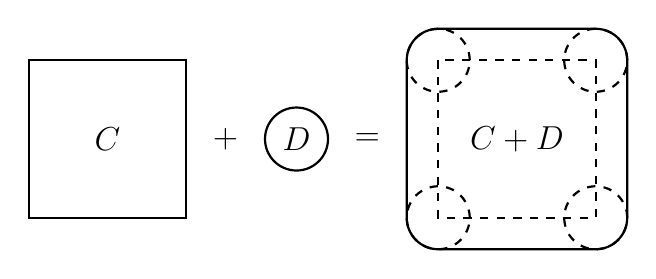
\begin{tikzpicture}
		%--shape C
		\draw[thick] (-1,1) rectangle (1,-1);
		\node at (0,0) {\large $C$};
		
		\node at (1.5,0) {\large $+$};
		%--shape D
		\draw[thick] (2.4,0) circle (0.4);
		\node at (2.4,0) {\large $D$};
		
		\node at (3.3,0) {\large $=$};
		%--shape of Mikowski sum (C+D)
		\draw[thick, dashed] (4.2,1) rectangle (6.2,-1);
		\foreach \x in {4.2, 6.2}
			\foreach \y in {-1,1}
				\draw[thick, dashed] (\x, \y) circle (0.4);
		\draw[rounded corners=0.4cm, thick] (3.8,1.4) rectangle (6.6,-1.4);
		\node at (5.2,0) {\large $C+D$};
	\end{tikzpicture}
	\caption{正方形和圆的Minkowski和是一个具有圆角的正方形.}
\end{figure}
\noindent
从这一定理出发, 很容易证明经典等周不等式: 记$\B^n$为$\mathbb{R}^n$中的单位球, 对任意$A \subseteq \mathbb{R}^n$满足$\vol(A) = \vol(\B^n)$, 
\begin{align*}
	(\vol(A^{\epsilon}))^{\frac1n}
	&= (\vol(A + \epsilon \B^n))^{\frac1n}
	= (1+\epsilon) \left(\vol\left(\frac{1}{1+\epsilon} A + \frac{\epsilon}{1+\epsilon} \B^n\right)\right)^{\frac1n} \\
	&\geq (\vol(A))^{\frac1n} + \epsilon (\vol(\B^n))^{\frac1n} 
	= (1+\epsilon) (\vol(\B^n))^{\frac1n} 
	= \left( \vol((\B^n)^{\epsilon}) \right)^{\frac1n}. 
\end{align*}

本节和下一节我们考虑度量空间$(\mathcal{X}, \rho)$中的集中不等式, 这需要对度量空间赋予一个概率测度$\mathbb{P}$, 我们称三元组$(\mathcal{X}, \rho, \mathbb{P})$为\textbf{度量测度空间}. 

等周不等式可以表述为确定满足$\mathbb{P}[A] \geq 1/2$、使得测度$\mathbb{P}[A^{\epsilon}]$最小的集合$A \subseteq \mathcal{X}$.
我们引入$(\mathcal{X}, \rho, \mathbb{P})$上的集中度函数$\alpha \colon \mathbb{R}_{\geq 0} \to [0, 1/2]$
\begin{equation*}
	\alpha_{\mathbb{P}}(\epsilon)
	:= \sup_{A \subseteq \mathcal{X} \colon \mathbb{P}[A] \geq 1/2} \left\{ 1 - \mathbb{P}[A^{\epsilon}] \right\}. 
\end{equation*}
于是等周不等式相当于确定$\alpha_{\mathbb{P}}$的上界. 

下面的定理说明, 集中度函数可以控制Lipschitz函数的尾部. 
回忆$f(X)$的\textbf{中位数}是指满足$\mathbb{P}[f(X) \geq m_f] \geq 1/2$, $\mathbb{P}[f(X) \leq m_f] \geq 1/2$的某个常数$m_f$. 

\begin{theorem}[Lévy不等式]
	设$f \colon \mathcal{X} \to \mathbb{R}$关于$\rho$是$L$-Lipschitz连续的函数, $X \sim \mathbb{P}$, 有$\mathbb{P}[ |f(X) - m_f| \geq \epsilon] \leq 2 \alpha(\epsilon / L)$. 
	特别地, 当$f$是Lipschitz连续函数时, 我们有
	\begin{equation*}
		\mathbb{P}[ |f(X) - m_f| \geq \epsilon] \leq 2 \alpha(\epsilon / L). 
	\end{equation*}
\end{theorem}
\begin{proof}
	令$A := \{x \in \mathcal{X} \colon f(x) \leq m_f\}$, 于是$\mathbb{P}[A] \geq 1/2$. 
	由扩张的定义, 对任意$x \in A^{\epsilon / L}$, 存在$y \in A$使得$\rho(x,y) < \epsilon / L$. 
	于是$f(x) < f(y) + |f(x) - f(y)| < m_f + \varepsilon$, 进一步地, 我们有$\mathbb{P}[A^{\epsilon / L}] \leq \mathbb{P}[f(X) < m_f + \epsilon]$. 
	取余集可以得到
	\begin{equation*}
		\mathbb{P}[f(X) \geq m_f + \epsilon] 
		\leq 1 - \mathbb{P}[A^{\epsilon / L}] 
		\leq \alpha_{\mathbb{P}}(\epsilon / L). 
	\end{equation*}
	对$-f$运用相同的方法可以得到下偏差不等式, 结合起来可得集中不等式. 
\end{proof}

反之, Lipschitz函数的集中不等式也蕴含着等周不等式, 于是两种t对尾部的控制是等价的. 

\begin{theorem}
	若存在函数$\beta \colon \mathbb{R}_{\geq 0} \to [0, 1]$使得对任意的$(\mathcal{X}, \rho)$上的Lipschitz函数都有
	\begin{equation*}
		\mathbb{P}[f(X) \geq \mathbb{E}f(X) + \epsilon] \leq \beta(\epsilon),\; \forall \epsilon \geq 0, 
	\end{equation*}
	那么$\alpha_{\mathbb{P}}(\epsilon) \leq \beta(\epsilon / 2)$. 
\end{theorem}
\begin{proof}
	对任意$\mathcal{X}$中满足$\mathbb{P}[A] \geq 1/2$的可测集$A$, 构造$f_A(x) := \rho(x, A) \wedge \epsilon$. 
	注意到在$A$上有$f_A = 0$, 在$A$外有$f_A \leq \epsilon$, 所以$\mathbb{E}f_A(X) \leq \epsilon (1 - \mathbb{P}[A]) \leq \epsilon / 2$. 
	于是我们有
	\begin{equation*}
		1 - \mathbb{P}[A^\epsilon]
		= \mathbb{P}[X \in \bar A^{\epsilon}]
		= \mathbb{P}[f_A(X) \geq \epsilon] 
		\leq \mathbb{P}\left[f_A(X) \geq \mathbb{E}f_A(X) + \frac{\epsilon}{2}\right]
		\leq \beta\left( \frac{\epsilon}{2} \right),  
	\end{equation*}
	再对满足条件$\mathbb{P}[A] \geq 1/2$的$A$取上确界即可. 
	其中最后一个不等式是由于$f_A$是一个Lipschitz函数: 
	\begin{itemize}
		\item 若$x, y \in A^{\epsilon}$, 则$|f_A(x) - f_A(y)| = |\rho(x, A) - \rho(y, A) | \leq  \rho(x, y)$; 
		\item 若$x, y \in \bar A^{\epsilon}$, 则$|f_A(x) - f_A(y)| = |\epsilon - \epsilon| = 0 \leq \rho(x, y)$;
		\item 若$x \in A^{\epsilon}$, $y \in \bar A^{\epsilon}$, 此时$\rho(x, A) \geq \rho(y, A) - \rho(x, y) \geq \epsilon - \rho(x, y)$, 则$|f_A(x) - f_A(y)| =  \epsilon - \rho(x, A) \leq \epsilon - (\epsilon - \rho(x, y)) = \rho(x, y)$.
	\end{itemize}
\end{proof}


%%%%%%%%%%%%%%%%%%%%%%%%%%%%%%%%%%%%%%%%%%%%%%%%%%%%%%%%%%%%%%%%%%%%%%
\subsection{传输成本不等式}

\subsubsection{Wasserstein距离}

给定$(\mathcal{X}, \rho)$上的两个概率分布$\mathbb{Q}$和$\mathbb{P}$, 它们之间由$\rho$诱导的\textbf{Wasserstein距离}为
\begin{equation*}
	W_{\rho}(\mathbb{Q}, \mathbb{P}) 
	:= \sup_{\|f\|_{\text{Lip}} \leq 1} \left\{ \mathbb{E}_{\mathbb{Q}} [f] - \mathbb{E}_{\mathbb{P}} [f] \right\}
	= \sup_{\|f\|_{\text{Lip}} \leq 1} \int f (\dd \mathbb{Q} - \dd \mathbb{P}). 
\end{equation*}
可以证明这样的$W_{\rho}$构成了一个度量. 
对任意耦合$\M \in \mathcal{C}(\mathbb{Q}, \mathbb{P})$, $f \colon \cX \to \mathbb{R}$为Lipschitz函数, 根据Fubini定理我们可以得到
\begin{equation*}
	\int \rho(x, x') \dd \M(x, x')
	\geq \int (f(x) - f(x')) \dd \M(x, x')
	= \int f(\dd \mathbb{P} - \dd \mathbb{Q}). 
\end{equation*}
\textbf{Kantorovich–Rubinstein对偶}告诉我们, 左侧关于耦合的下确界和右侧关于Lipschitz函数的上界是相等的, 即有
\begin{equation*}
	W_{\rho}(\mathbb{Q}, \mathbb{P})
	= \inf_{\M \in \mathcal{C}(\mathbb{Q}, \mathbb{P})} \mathbb{E}_{\M} \left[ \rho \right]
	= \inf_{\M \in \mathcal{C}(\mathbb{Q}, \mathbb{P})} \int_{\mathcal{X} \times \mathcal{X}} \rho(x, x') \dd \M(x, x'). 
\end{equation*}
于是Wasserstein距离也被称为\textbf{推土机距离}: 两个土堆的形状(分布$\mathbb{P}, \mathbb{Q}$)确定, 传输成本(距离$\rho$)确定, Wasserstein距离就是最优的搬运方案(最优的耦合$\M \in \mathcal{C}(\mathbb{Q}, \mathbb{P})$)下的传输成本, 等式右侧关于耦合的优化被称为最优传输问题. 

\begin{example}[Hamming度量和全变差距离]\label{ex:HammingMetricAndTVDistance}
	关于Hamming度量的Wasserstein距离$W_{\text{Ham}}(\mathbb{Q}, \mathbb{P})$等价于全变差距离$\|\mathbb{Q} - \mathbb{P}\|_{\text{TV}} := \sup_{A \subseteq \mathcal{X}} |\mathbb{Q}(A) - \mathbb{P}(A)|$, 再由Kantorovich–Rubinstein对偶, 我们有
	\begin{equation*}
		\|\mathbb{Q} - \mathbb{P}\|_{\text{TV}}
		= \inf_{\M \in \mathcal{C}(\mathbb{Q}, \mathbb{P})} \int_{\cX \times \cX} \I{\{x \neq x'\}} \dd \M(x, x')
		= \inf_{\M \in \mathcal{C}(\mathbb{Q}, \mathbb{P})} \M[Y \neq X], 
	\end{equation*}
	其中$X \sim \mathbb{P}$, $Y \sim \mathbb{Q}$. 
	\begin{proof}
	函数$f$关于Hamming度量Lipschitz连续等价于$f$值域在某个区间$[c, c+1]$中, 不失一般性地, 我们假定$c = 0$. 
	记$\mathbb{Q}$和$\mathbb{P}$关于测度$\nu$的密度\footnote{这样的测度$\nu$是存在的, 例如$\mathbb{P}$和$\mathbb{Q}$都关于$(\mathbb{P} + \mathbb{Q})/2$绝对连续.}分别为$q$, $p$, 集合$A = \{x \in \mathcal{X} \colon q(x) \geq p(x)\} $, 于是有
	\begin{equation*}
		W_{\text{Ham}}(\mathbb{Q}, \mathbb{P})
		= \sup_{f \colon \mathcal{X} \to [0, 1]} \int_{\mathcal{X}} f (q - p) \dd \nu 
		\leq \int_A (\dd \mathbb{Q} - \dd \mathbb{P})
		\leq \|\mathbb{Q} - \mathbb{P}\|_{\text{TV}}. 
	\end{equation*}
	另一方面, 对任意可测集$B \subseteq \mathcal{X}$, 注意到示性函数$\mathbb{I}_B$是Lipschitz连续的, 于是
	\begin{equation*}
		\mathbb{Q}(B) - \mathbb{P}(B) 
		= \int \mathbb{I}_B (\dd \mathbb{Q} - \dd \mathbb{P}) 
		\leq W_{\text{Ham}}(\mathbb{Q}, \mathbb{P}). 
	\end{equation*}
	于是有$\|\mathbb{Q} - \mathbb{P}\|_{\text{TV}} \leq W_{\text{Ham}}(\mathbb{Q}, \mathbb{P})$, 从而二者等价. 
	\end{proof}
\end{example}

\subsubsection{KL散度与传输成本不等式}

 $\mathbb{Q}$和$\mathbb{P}$之间的\textbf{Kullback–Leibler散度}(亦称相对熵)定义为
\begin{equation}
	D(\mathbb{Q} \| \mathbb{P})
	:= \begin{cases}
		\mathbb{E}_{\mathbb{Q}} \left[ \log \frac{\dd \mathbb{Q}}{\dd \mathbb{P}} \right]
		= \int_{\mathcal{X}} q(x) \log \frac{q(x)}{p(x)} \nu(\dd x), & \mathbb{Q} \ll \mathbb{P}, \\
		+\infty, &\text{其它}. 
	\end{cases} 
\end{equation}
其中$q, p$为$\mathbb{Q}, \mathbb{P}$的密度, $\nu$为$\mathcal{X}$上的Lebesgue测度. 
尽管KL散度可以描述分布间的差异, 它实际上并不是一个度量: 它不满足对称性和三角不等式. 

称$(\mathcal{X}, \rho)$上的概率测度$\mathbb{P}$满足参数为$\gamma > 0$的\textbf{$\rho$-传输成本不等式}, 如果对任意的概率测度$\mathbb{Q}$总有
 \begin{equation}\label{eq:TransportationCostInequality}
 	W_{\rho} (\mathbb{Q}, \mathbb{P}) \leq \sqrt{2 \gamma D(\mathbb{Q} \| \mathbb{P})}.
 \end{equation}
 这样的不等式在信息论中也被称为\textbf{信息不等式}, 例如经典的Pinsker–Csiszár–Kullback不等式: 对任意分布$\Q$, $\P$, 
 \begin{equation}\label{eq:Pinsker–Csiszár–Kullback}
 	\|\Q - \P\|_{\text{TV}} \leq \sqrt{\frac{1}{2}D(\Q\|\P)}, 
 \end{equation}
 结合示例\ref{ex:HammingMetricAndTVDistance}, 这实际上是说任意分布$\P$都满足参数$\gamma = \frac{1}{4}$的Hamming度量传输成本不等式. 
下述定理告诉我们, 在控制Lipschitz函数的矩生成函数时, 传输成本不等式成立. 

\begin{theorem}[Bobkov-Götze]\label{thm:Bobkov-Götze}
	设度量空间$\cX, \rho$上的随机变量$X \sim \mathbb{P}$, 下列命题等价: 
	\begin{enumerate}
		\item 对任意Lipschitz连续的函数$f$, $f(X)$是$\sigma$-次高斯的;
		\item 概率测度$\mathbb{P}$满足参数为$\sigma^2$的$\rho$-传输不等式, 即对任意概率测度$\mathbb{Q}$均成立
			\begin{equation*}
				W_{\rho}(\mathbb{Q}, \mathbb{P}) \leq \sqrt{2 \sigma^2 D(\mathbb{Q} \| \mathbb{P})}. 
			\end{equation*}
	\end{enumerate}
\end{theorem}

证明的关键在于注意到相对熵和矩生成函数间的密切关系, 下述的结果可以追溯到统计力学最早的历史. 
\begin{lemma}[Gibbs变分原理]\label{lemma:GibbsVariation}
	\begin{equation*}
		\log \mathbb{E}_{\mathbb{P}}[\mathrm{e}^f] = \sup_{\mathbb{Q}} \left\{ \mathbb{E}_{\mathbb{Q}} [f] - D(\mathbb{Q} \| \mathbb{P}) \right\}
	\end{equation*}
\end{lemma}
\begin{proof}
	这里我们假定$f$有界来避免可积性的问题(否则, 考虑$f \wedge M$的结果, 再对$M$取上确界即可). 
	考虑测度$\tilde{\mathbb{P}}$, 它关于$\mathbb{P}$的Radon–Nikodym导数为$\frac{\mathrm{e}^{f}}{\mathbb{E}_{\mathbb{P}}[\mathrm{e}^{f}]}$, 当$\mathbb{Q} \ll \mathbb{P}$时, 
	\begin{align*}
		\log \mathbb{E}_{\mathbb{P}}[\mathrm{e}^f] - D(\mathbb{Q} \| \tilde{\mathbb{P}})
		&= \log \mathbb{E}_{\mathbb{P}}[\mathrm{e}^f] - \int \log \frac{\dd \mathbb{Q}}{\dd \tilde{\mathbb{P}}} \dd \mathbb{Q} \\
		&= \log \mathbb{E}_{\mathbb{P}}[\mathrm{e}^f] - \int \log \frac{\dd \mathbb{Q}}{\dd \mathbb{P}} \dd \mathbb{Q} + \int \log \frac{\dd \mathbb{Q}}{\dd \tilde{\mathbb{P}}} \dd \mathbb{Q} \\
		&= \mathbb{E}_{\mathbb{Q}}[f] - D(\mathbb{Q} \| \mathbb{P}). 
	\end{align*}
	于是两侧关于$\mathbb{Q}$的上确界相同, 特别是左侧中$- D(\mathbb{Q} \| \tilde{\mathbb{P}})$关于$\mathbb{Q}$的上确界为$0$.   
\end{proof}

\begin{proof}[\keben 定理\ref{thm:Bobkov-Götze}的证明]
	由定义, 条件(1)等价于
	\begin{equation*}
		\log \mathbb{E}_{\mathbb{P}} [\exp(\lambda(f - \mathbb{E}_{\mathbb{P}}[f]))] \leq \frac{\lambda^2 \sigma^2}{2}, 
		\quad \forall \lambda \in \mathbb{R},\; \|f\|_{\text{Lip}} \leq 1. 
	\end{equation*}
	结合引理\ref{lemma:GibbsVariation}, 这等价于
	\begin{equation*}
		\sup_{\lambda \in \mathbb{R}} \sup_{\|f\|_{\text{Lip} \leq 1}} \sup_{\mathbb{Q}} \left\{\lambda(\mathbb{E}_{\mathbb{Q}}[f] - \mathbb{E}_{\mathbb{P}}[f]) - D(\mathbb{Q} \| \mathbb{P}) -  \frac{\lambda^2 \sigma^2}{2} \right\} \leq 0. 
	\end{equation*}
	交换上确界的顺序并求出关于$f$和$\lambda$的上确界, 我们可以得到(2)的等价表述: 
	\begin{equation*}
		\sup_{\mathbb{Q}} \left\{\frac{W_{\rho}(\mathbb{Q}, \mathbb{P})^2}{2 \sigma^2} - D(\mathbb{Q} \| \mathbb{P}) \right\} \leq 0
	\end{equation*}
\end{proof}

\subsubsection{传输成本的张量化}
定理\ref{thm:Bobkov-Götze}描述了任意度量空间$(\cX, \rho)$上Lipschitz函数的次高斯性质, 但这并不是一个高维的结果, 而推广至高维的关键思想是张量化. 
在此之前, 我们先介绍KL散度的链法则. 
\begin{lemma}[Kullback–Leibler散度的链法则]\label{lemma:ChainRuleForKLDivergence}
	给定两个$n$维分布$\mathbb{Q} \ll \mathbb{P}$, 它们之间的KL散度可以分解为
	\begin{equation*}
		D(\mathbb{Q} \| \mathbb{P})
		= D(\mathbb{Q}_1 \| \mathbb{P}_1) + \sum_{j=2}^n \mathbb{E}_{\mathbb{Q}_1^{j-1}} \left[ D\left(\mathbb{Q}_{j | j-1}(\;\cdot\; | \bm{X}_1^{j-1}) \big\| \mathbb{P}_{j | j-1}(\;\cdot\; | \bm{X}_1^{j-1})\right) \right], 
	\end{equation*}
	其中$\mathbb{Q}_j, \mathbb{P}_j$分别为$\mathbb{Q}, \mathbb{P}$关于第$j$个分量的边缘分布, $\mathbb{Q}_{j | j-1}, \mathbb{P}_{j | j-1}$分别为给定前$j-1$维随机变量下, $\mathbb{Q}, \mathbb{P}$关于第$j$维的条件分布. 
\end{lemma}
\begin{proof}
	我们只说明$n = 2$的情形, 更高维的结果可以通过归纳法得到. 
	记$\mathbb{Q}$和$\mathbb{P}$关于测度$\nu$的密度分别为$q$, $p$, 
	\begin{align*}
		& D(\mathbb{Q} \| \mathbb{P})
		= \int q(x_1, x_2) \log \frac{q(x_1, x_2)}{p(x_1, x_2)} \dd \nu(x_1, x_2) \\
		=& \int q_1(x_1) q_{2|1}(x_2|x_1) \log \frac{q_1(x_1) q_{2|1}(x_2|x_1)}{p_1(x_1) p_{2|1}(x_2|x_1)} \dd \nu(x_1, x_2) \\
		=& \int q_1(x_1) \log \frac{q_1(x_1)}{p_1(x_1)} \dd \nu_1(x_1) + \int q_1(x_1) \int q_{2|1}(x_2|x_1) \log \frac{q_{2|1}(x_2|x_1)}{p_{2|1}(x_2|x_1)} \dd \nu(x_1, x_2) \\
		=& D(\mathbb{Q}_1 \| \mathbb{P}_1) + \mathbb{E}_{\Q_1} \left[ D\left(\Q_{2|1}(\;\cdot\; | \bm{X}_1) \| \P_{2|1}(\;\cdot\; | \bm{X}_1)\right) \right]. 
	\end{align*}
\end{proof}

\begin{proposition}[传输成本不等式的张量化]\label{thm:TensorizationForTransportationCost}
	若对于每个$k = 1, \dots, n$, 度量空间$\cX$上的概率测度$\mathbb{P}_k$满足参数为$\gamma_k$的$\rho_k$-传输成本不等式, 那么乘积空间$\cX^n$上的乘积测度$\mathbb{P} := \otimes_{k=1}^n \mathbb{P}_k$满足传输成本不等式
	\begin{equation}
		W_{\rho}(\mathbb{Q}, \mathbb{P})
		\leq \sqrt{2 \left(\sum_{k=1}^n \gamma_k \right) D(\mathbb{Q} \| \mathbb{P})}, \quad \text{对任意$\cX^n$上的分布$\mathbb{Q}$,}
	\end{equation}
	其中$\rho(x, y) := \sum_{k=1}^n \rho_k(x_k, y_k)$. 
\end{proposition}
\begin{proof}
	由Kantorovich–Rubinstein对偶, 只需说明对任意$\cX^n$上的分布$\mathbb{Q}$, 存在某个耦合$\M \in \mathcal{C}(\mathbb{Q}, \mathbb{P})$使得不等式$\mathbb{E}_{\M}[\rho] \leq \sqrt{2 \left(\sum_k \gamma_k \right) D(\mathbb{Q} \| \mathbb{P})}$成立. 
	我们用归纳法证明这样的分布$\M$的存在性. 
	
	考虑随机变量 $(\bm{X}_1^n, \bm{Y}_1^n) \sim \M$, 对于$j = 1, \dots, n$, 记$\M_j$为$(X_j, Y_j)$的边缘分布. 
	特别地, $\M_1 \in \mathcal{C}(\mathbb{Q}_1, \mathbb{P}_1)$为最佳耦合, 即有
	\begin{equation*}
		\mathbb{E}_{\M_1} [\rho_1] = W_{\rho_1} (\mathbb{Q}_1, \mathbb{P}_1) \leq \sqrt{2 \gamma_1 D(\mathbb{Q}_1 \| \mathbb{P}_1)}. 
	\end{equation*}
	记$\M_1^j$为$(\bm{X}_1^j, \bm{Y}_1^j)$的联合分布, $\M_{j | j-1}$为给定$(\bm{X}_1^{j-1}, \bm{Y}_1^{j-1})$下$(X_j, Y_j)$的条件分布. 
	现在假定我们得到了满足不等式
	\begin{equation*}
		\mathbb{E}_{\M_1^{j-1}} \left[\sum_{k=1}^{j-1} \rho_k \right]
		\leq \sqrt{2 \left(\sum_{k=1}^{j-1} \gamma_k \right) D(\mathbb{Q}_1^{j-1} \| \mathbb{P}_1^{j-1})}
	\end{equation*}
	的耦合$\M_1^{j-1}$, 由条件, 存在$\left(\mathbb{Q}_{j | j-1}(\;\cdot\; | \bm{x}_1^{j-1}), \mathbb{P}_j\right)$的耦合$\M_{j | j-1}(\;\cdot\; | \bm{x}_1^{j-1}, \bm{y}_1^{j-1})$使得
	\begin{equation*}
		\mathbb{E}_{\M_{j | j-1}}[ \rho_j] 
		\leq \sqrt{2 \gamma_j D\left(\mathbb{Q}_{j | j-1}(\;\cdot\; | \bm{x}_1^{j-1}) \| \mathbb{P}_j\right)}, 
		\quad \forall \bm{x}_1^{j-1} \in \cX^{j-1}, 
	\end{equation*}
	于是利用条件期望的塔形性质, 由平方根函数的凹性和Jensen不等式、Cauchy-Schwarz不等式、KL散度的链法则, 可以得到
	\begin{align*}
		& \mathbb{E}_{\M}[\rho]
		= \sum_{k=1}^n \mathbb{E}_{\M}[ \rho_k]
		= \mathbb{E}_{\M_1}[\rho_1] + \sum_{j=2}^n \mathbb{E}_{\M_1^{j-1}} \left[ \mathbb{E}_{\M_{j | j-1}} [\rho_j] \right] \\
		\leq & \sqrt{2 \gamma_1 D(\mathbb{Q}_1 \| \mathbb{P}_1)} + \sum_{j=2}^n \sqrt{2 \gamma_j \mathbb{E}_{\M_1^{j-1}} \left[ D\left(\mathbb{Q}_{j | j-1}(\;\cdot\; | \bm{X}_1^{j-1}) \| \mathbb{P}_j\right) \right]} \\
		\leq & \sqrt{2 \left(\sum_{k=1}^n \gamma_k \right)} \sqrt{D(\mathbb{Q}_1 \| \mathbb{P}_1) + \sum_{j=2}^n \mathbb{E}_{\M_1^{j-1}} \left[ D\left(\mathbb{Q}_{j | j-1}(\;\cdot\; | \bm{X}_1^{j-1}) \| \mathbb{P}_j\right) \right]} \\
		= & \sqrt{2 \left(\sum_{k=1}^n \gamma_k \right) D(\mathbb{Q} \| \mathbb{P})}. 
	\end{align*}
\end{proof}

 
\begin{example}[有界差不等式']
	下面我们利用张量化的传输成本不等式重新得到推论\ref{cor:BddDiffIneq}.
	设函数$f \colon \cX^n \to \mathbb{R}$满足参数为$(L_1, \dots, L_n)$的有界差不等式, 利用三角不等式可以得到, $f$关于重尺度化的Hamming度量$\rho(x, y) := \sum_k L_k \I{\{x_k \neq y_k\}}$是Lipschitz连续的. 
	于是由不等式\ref{eq:Pinsker–Csiszár–Kullback}, 每个边缘分布$\P_k$满足参数为$\gamma_k = L_k^2 / 4$的$L_k \I{\{x_k \neq y_k\}}$-传输成本不等式. 
	结合定理\ref{thm:TensorizationForTransportationCost}和定理\ref{thm:Bobkov-Götze}, Lipschitz函数$f$是$\sqrt{\sum_k L_k^2} / 2$-次高斯的. 
\end{example}


 
\begin{theorem}
	若度量测度空间$(\mathcal{X}, \rho, \mathbb{P})$中的概率测度满足$\rho$-传输成本不等式\eqref{eq:TransportationCostInequality}, 那么它的集中度满足
	\begin{equation}\label{eq:ConcetrationByTransportationCost}
		\alpha_{\mathbb{P}}(\epsilon) \leq 2 \exp \left(- \frac{\epsilon^2}{2 \gamma} \right).
	\end{equation}
\end{theorem}
\begin{proof}
	考虑任意满足$\mathbb{P}[A] \geq \frac12$的集合$A$和$\epsilon > 0$, 只需证明$B := \bar A^{\epsilon}$的测度总是小于不等式\eqref{eq:ConcetrationByTransportationCost}的右侧. 
	若$\mathbb{P}[B] = 0$, 则不等式显然成立, 下面我们总假设$\mathbb{P}[B] > 0$. 
	
	考虑$\mathbb{P}_A$, $\mathbb{P}_B$为在$A$和$B$上的条件分布, $\M$为它们的任意耦合, 于是
	\begin{align*}
		\int_{\mathcal{X} \times \mathcal{X}} \rho(x, x') \dd \M(x, x')
		&= \int_{A \times B} \rho(x, x') \dd \M(x, x') \\
		&\geq \rho(A, B) \int_{A \times B} \dd \M 
		= \rho(A, B) 
		\geq \epsilon. 
	\end{align*}
	对所有可能的耦合取下确界, 可得$W_{\rho}(A, B) \geq \epsilon$. 
	再由三角不等式和$\rho$-传输成本不等式, 我们有(这里根号下似乎少了个2)
	\begin{align*}
		\epsilon 
		&\leq W_{\rho}(\mathbb{P}, \mathbb{P}_A) + W_{\rho}(\mathbb{P}, \mathbb{P}_B) 
		\leq \sqrt{\gamma D(\mathbb{P}_A \| \mathbb{P})} + \sqrt{\gamma D(\mathbb{P}_B \| \mathbb{P})} \\
		&\leq \sqrt{2 \gamma} \left[ D(\mathbb{P}_A \| \mathbb{P}) + D(\mathbb{P}_B \| \mathbb{P}) \right]^{1/2}.
	\end{align*}
	另一方面, $\mathbb{P}_A$的密度为$p_A(x) = \frac{p(x) \mathbb I_A(x)}{\mathbb{P}[A]}$, 于是$D(\mathbb{P}_A \| \mathbb{P}) = - \log \mathbb{P}[A]$, $D(\mathbb{P}_B \| \mathbb{P}) = -\log \mathbb{P}[B]$, 从而有$\epsilon^2 \leq -  2 \gamma \log (\mathbb{P}[A] \mathbb{P}[B])$, 等价地
	\begin{equation*}
		 \mathbb{P}[B] 
		 \leq (\mathbb{P}[A])^{-1} \exp\left(- \frac{\epsilon^2}{2 \gamma} \right) 
		 \leq 2 \exp\left(- \frac{\epsilon^2}{2 \gamma} \right). 
	\end{equation*}
\end{proof}



\subsubsection{非对称耦合成本}

定义
\begin{align*}
	\mathcal{C}(\mathbb{Q}, \mathbb{P})
	= \sqrt{\int\left(1 - \frac{\dd \mathbb{Q}}{\dd \mathbb{P}} \right)_+^2 \dd \mathbb{P}}
\end{align*}




















